%% Hapax: Fusing Dependent Tensor Reductions by Deriving Single-Pass Reducers
%% PLDI 2027 submission (PACMPL, acmsmall). Build: bash build.sh
%% Every number in the text comes from gen/stats.tex (generated from data/*.json);
%% hand-written numbers carry a "% src:" comment.
\PassOptionsToPackage{table}{xcolor}
\documentclass[acmsmall,screen,review,anonymous,nonacm]{acmart}

\citestyle{acmnumeric}
% Packages. acmart already loads amsmath, amsthm, booktabs, natbib, hyperref,
% xcolor, graphicx, caption and microtype: do not load them again.
\usepackage{mathtools}
\usepackage{stmaryrd}            % \llbracket \rrbracket
\usepackage{xspace}
\usepackage{array}
\usepackage{multirow}
\usepackage{subcaption}
\usepackage{wrapfig}
\usepackage{pifont}              % \ding{51} check, \ding{55} cross
\usepackage{listings}
\usepackage{tikz}
\usetikzlibrary{arrows.meta,positioning,fit,calc,backgrounds,shapes.misc,decorations.pathreplacing,patterns}
\usepackage{pgfplots}
\pgfplotsset{compat=1.18}
\usepackage[ruled,linesnumbered,noend]{algorithm2e}
\usepackage{cleveref}            % after hyperref (loaded by acmart)
\crefname{section}{Section}{Sections}
\Crefname{section}{Section}{Sections}
\crefname{figure}{Fig.}{Figs.}
\Crefname{figure}{Figure}{Figures}
\crefname{table}{Table}{Tables}
\crefname{algocf}{Algorithm}{Algorithms}
\crefname{algorithm}{Algorithm}{Algorithms}
\Crefname{algocf}{Algorithm}{Algorithms}
\crefname{lstlisting}{Listing}{Listings}
\crefname{listing}{Listing}{Listings}
\Crefname{listing}{Listing}{Listings}
\crefname{theorem}{Theorem}{Theorems}
\crefname{lemma}{Lemma}{Lemmas}
\crefname{proposition}{Proposition}{Propositions}
\crefname{definition}{Definition}{Definitions}
\crefname{example}{Example}{Examples}
\crefname{corollary}{Corollary}{Corollaries}
\crefname{equation}{Eq.}{Eqs.}
\crefname{appendix}{Appendix}{Appendices}


% Keep half-width diagrams/algorithms beside their explanatory prose without reordering the argument.
\newenvironment{paperdiagram}{\begin{minipage}[t]{0.48\linewidth}\vspace{0pt}}{\end{minipage}}

% Reserve room for a wrapped diagram; its accompanying prose remains pageable.
\newcommand{\reservewrapspace}[1]{%
  \par\penalty-100\relax\begingroup
  \dimen0=#1\relax
  \dimen2=\pagegoal\advance\dimen2 by -\pagetotal
  \ifdim\dimen0>\dimen2\newpage\fi
  \endgroup
}

% Clear any remaining wrapped height before a full-width theorem or display.
% wrapfig counts the remaining narrow lines plus one; clearing alone adds no space.
\newcommand{\finishwrapspace}{%
  \par
  \ifnum\value{WF@wrappedlines}>1\relax
    \vspace{\dimexpr\value{WF@wrappedlines}\baselineskip-\baselineskip\relax}%
  \fi
  \WFclear
}

% Chinese text only; keep acmart's geometry, Latin fonts, math and float styles.
\usepackage{xeCJK}
\setCJKmainfont{FandolSong-Regular.otf}[
  BoldFont=FandolSong-Bold.otf,
  ItalicFont=FandolKai-Regular.otf]
\setCJKsansfont{FandolHei-Regular.otf}[BoldFont=FandolHei-Bold.otf]
\setCJKmonofont{FandolFang-Regular.otf}

% xspace knows Latin punctuation; teach it the corresponding Chinese marks.
\xspaceaddexceptions{，。；：、！？）】》”’}

% Colours: one meaning each, used in figures, equations and captions alike
% (Okabe-Ito, distinguishable in grayscale by the line style that goes with it).
\definecolor{origblue}{HTML}{0072B2}   % the original program, original values
\definecolor{staleorange}{HTML}{D55E00} % stale or wrong values (naive fusion)
\definecolor{fixgreen}{HTML}{009E73}   % values corrected by the derived join
\definecolor{auxpurple}{HTML}{8E5AA8}  % states the program does not compute
\definecolor{boxgray}{HTML}{F2F2F2}
\definecolor{rulegray}{HTML}{8C8C8C}
\definecolor{codebg}{HTML}{F7F7F7}
\definecolor{kwgreen}{HTML}{1B7837}
\definecolor{strred}{HTML}{B2182B}
\definecolor{cmtgray}{HTML}{6E6E6E}

\newcommand{\orig}[1]{\textcolor{origblue}{#1}}
\newcommand{\stale}[1]{\textcolor{staleorange}{#1}}
\newcommand{\fix}[1]{\textcolor{fixgreen}{#1}}
\newcommand{\aux}[1]{\textcolor{auxpurple}{#1}}

% TikZ styles
\tikzset{
  >={Stealth[length=2mm]},
  artifact/.style={draw, rounded corners=2pt, fill=white, font=\sffamily\small,
    inner sep=3pt, align=center},
  stage/.style={draw, rounded corners=2pt, fill=boxgray, font=\sffamily\small,
    inner sep=4pt, align=center, minimum height=7mm},
  future/.style={draw, dashed, rounded corners=2pt, font=\sffamily\small,
    inner sep=4pt, align=center, text=rulegray},
  flow/.style={->, thick, draw=origblue},
  weak/.style={->, densely dashed, draw=rulegray},
  cell/.style={draw, minimum width=7mm, minimum height=6mm, font=\small, inner sep=1pt},
  tmpcell/.style={cell, densely dashed},
  lbl/.style={font=\sffamily\scriptsize, text=cmtgray},
}

% Code listings (TE is Python)
\lstdefinestyle{te}{
  language=Python,
  basicstyle=\ttfamily\scriptsize,
  keywordstyle=\color{kwgreen}\bfseries,
  stringstyle=\color{strred},
  commentstyle=\color{cmtgray},
  morekeywords={te,tir},
  columns=fullflexible,
  keepspaces=true,
  breaklines=true,
  breakatwhitespace=false,
  postbreak=\mbox{\textcolor{rulegray}{$\hookrightarrow$}\space},
  showstringspaces=false,
  frame=tb,
  framerule=0.4pt,
  rulecolor=\color{rulegray},
  aboveskip=2pt,
  belowskip=2pt,
  xleftmargin=2pt,
  numbers=none,
  escapeinside={(*@}{@*)},
}
\lstset{style=te}

% algorithm2e: procedure names in small caps, as in the reference papers
\SetKwProg{Fn}{function}{}{}
\SetFuncSty{textsc}
\SetArgSty{textup}
\DontPrintSemicolon


% Illustrative program forms use the Listing counter, separately from method algorithms.
\lstdefinestyle{pseudocode}{
  style=te,
  language={},
  basicstyle=\small\rmfamily,
  keywordstyle=\bfseries,
  morekeywords={for,return,function},
  mathescape=true,
  captionpos=t,
  numbers=none,
  xleftmargin=0pt,
}

% ---------------------------------------------------------------- names
\newcommand{\sys}{Hapax\xspace}
\newcommand{\Neptune}{Neptune\xspace}
\newcommand{\RedFuser}{RedFuser\xspace}
\newcommand{\TE}{TE\xspace}
\newcommand{\code}[1]{\texttt{\small #1}}
\newcommand{\commreducer}{\code{te.comm\_reducer}\xspace}

% ---------------------------------------------------------------- notation
\newcommand{\Ax}{J}                       % the reduction axis
\newcommand{\pa}{A}                       % parts
\newcommand{\pb}{B}
\newcommand{\dunion}{\uplus}
\newcommand{\st}{I}                       % state map S -> I(S)
\newcommand{\Mrg}{\operatorname{join}}
\newcommand{\ident}{e}
\newcommand{\leaf}{L}
\newcommand{\epi}{E}
\newcommand{\red}{\oplus}
\newcommand{\ctx}{\kappa}
\newcommand{\cnt}{n}
\newcommand{\Judged}{\mathcal{A}}         % the judgement's tuple of reductions
\newcommand{\Own}{\mathcal{B}}            % the program's own loop results
\newcommand{\Cls}[1]{\mathcal{C}_{\mathrm{#1}}}
\newcommand{\R}{\mathbb{R}}
\newcommand{\sem}[1]{\llbracket #1 \rrbracket}
\newcommand{\maxop}{\operatorname{max}}
\newcommand{\Sum}{\textstyle\sum}
\DeclareMathOperator*{\bigred}{\bigoplus}

% ---------------------------------------------------------------- marks
\newcommand{\cmark}{\textcolor{fixgreen}{\ding{51}}}
\newcommand{\xmark}{\textcolor{staleorange}{\ding{55}}}
\newcommand{\pmark}{\textcolor{rulegray}{$\circ$}}       % partial
\newcommand{\nr}{\textcolor{rulegray}{n.r.}}            % not reported
\newcommand{\markRefused}{\textcolor{staleorange}{\ding{55}}}
\newcommand{\markFrontend}{\textcolor{rulegray}{\ding{55}}}
\newcommand{\tagP}{\textsc{p}}            % proven
\newcommand{\tagM}{\textsc{m}}            % measured
\newcommand{\tagS}{\textsc{s}}            % sampled

% ---------------------------------------------------------------- drafting
\newif\ifperf          % \perftrue once GPU numbers exist (Section 8.5, 7.2)
\perffalse
\newif\ifsubmit
\submitfalse
\newcounter{placeholders}
\newcommand{\placeholder}[1]{%
  \stepcounter{placeholders}%
  \ifsubmit\errmessage{placeholder left in a submission build: #1}\fi
  \par\noindent\fcolorbox{staleorange}{white}{\parbox{\dimexpr\linewidth-2\fboxsep-2\fboxrule}{%
    \small\textcolor{staleorange}{\textbf{Placeholder.}} #1}}\par}
\newcommand{\todo}[1]{\textcolor{staleorange}{[\textbf{TODO}: #1]}}

\submitfalse

% generated by Hapax/scripts/gen_tex.py -- do not edit
\newcommand{\dataCommit}{6c46fb1b02\xspace}
%   src: data/fused_ops.json meta.commit
\newcommand{\dataStale}{false\xspace}
%   src: meta.commit of every data/*.json vs HEAD
\newcommand{\pythonVersion}{3.12.14\xspace}
%   src: fused_ops.json meta.python
\newcommand{\sympyVersion}{1.14.0\xspace}
%   src: fused_ops.json meta.sympy
\newcommand{\zThreeVersion}{5.3.3\xspace}
%   src: fused_ops.json meta.z3
\newcommand{\cvcFiveVersion}{1.4.2\xspace}
%   src: fused_ops.json meta.cvc5
\newcommand{\nRegistry}{51\xspace}
%   src: fused_ops.json meta.registry (len(OPERATORS))
\newcommand{\nFusible}{44\xspace}
%   src: fused_ops.json meta.registry_fusible
\newcommand{\nFused}{42\xspace}
%   src: fused_ops.json: rows with fused = true
\newcommand{\nNegative}{7\xspace}
%   src: registry minus fusible
\newcommand{\nChains}{45\xspace}
%   src: fused_ops.json: chains over fused rows
\newcommand{\nPassesBefore}{117\xspace}
%   src: sum of passes_before
\newcommand{\nPassesAfter}{45\xspace}
%   src: sum of passes_after
\newcommand{\nPassesEqualHand}{42\xspace}
%   src: rows with passes_after == passes_hand
\newcommand{\nStates}{162\xspace}
%   src: sum of len(chain.states)
\newcommand{\nDerived}{49\xspace}
%   src: sum of len(chain.auxiliaries)
\newcommand{\nDerivedOps}{26\xspace}
%   src: rows with a non-empty auxiliaries list
\newcommand{\nCountOnlyOps}{0\xspace}
%   src: rows whose only auxiliary is count
\newcommand{\nMoreAuxOps}{26\xspace}
%   src: derived-ops minus count-only
\newcommand{\nNoAuxOps}{16\xspace}
%   src: fused rows without auxiliaries
\newcommand{\nAddedCount}{0\xspace}
%   src: auxiliaries named count
\newcommand{\nAddedR}{34\xspace}
%   src: auxiliaries ending .r<k> (supplemented coefficients)
\newcommand{\nAddedH}{6\xspace}
%   src: auxiliaries ending .h<k> (hoisted coefficients)
\newcommand{\nAddedM}{0\xspace}
%   src: auxiliaries ending .m<k> (parts of a max)
\newcommand{\nSupplement}{43\xspace}
%   src: selection steps with action supplement
\newcommand{\nPromote}{0\xspace}
%   src: selection steps with action promote
\newcommand{\nHoist}{6\xspace}
%   src: selection steps with action hoist
\newcommand{\nParts}{0\xspace}
%   src: selection steps with action parts
\newcommand{\nSplit}{0\xspace}
%   src: selection steps with action split
\newcommand{\nNoStep}{19\xspace}
%   src: chains with no selection step
\newcommand{\nStatesEqualJudged}{45\xspace}
%   src: chains with len(states) == theory_states
\newcommand{\nStatesBelowJudged}{0\xspace}
%   src: chains with len(states) < theory_states
\newcommand{\nStatesAboveJudged}{0\xspace}
%   src: chains with len(states) > theory_states
\newcommand{\nMechRebase}{16\xspace}
%   src: fused rows whose heaviest step is rebase
\newcommand{\nMechSupplement}{20\xspace}
%   src: fused rows whose heaviest step is supplement
\newcommand{\nMechPromote}{0\xspace}
%   src: fused rows whose heaviest step is promote
\newcommand{\nMechParts}{0\xspace}
%   src: fused rows whose heaviest step is parts
\newcommand{\nMechHoist}{6\xspace}
%   src: fused rows whose heaviest step is hoist
\newcommand{\nDomains}{7\xspace}
%   src: info_en.py domains of fused rows, excluding Constructed
\newcommand{\nShowcase}{17\xspace}
%   src: all selected showcase rows, including failures
\newcommand{\nShowFused}{17\xspace}
%   src: successfully fused showcase rows
\newcommand{\ratioCentredMedian}{1.20\xspace}
%   src: median err_synth[0]/err_unfused[0]
\newcommand{\ratioCentredMin}{0.23\xspace}
%   src: min of the same
\newcommand{\ratioCentredMax}{9.7\xspace}
%   src: max of the same
\newcommand{\nRatioCentredLeOne}{20\xspace}
%   src: count ratio_c <= 1
\newcommand{\nRatioCentredLeTwo}{30\xspace}
%   src: count ratio_c <= 2
\newcommand{\nRatioCentredLeFive}{40\xspace}
%   src: count ratio_c <= 5
\newcommand{\nRatioCentred}{42\xspace}
%   src: operators with a centred ratio
\newcommand{\ratioOffsetMedian}{1.06\xspace}
%   src: median err_synth[1]/err_unfused[1] (both > 0)
\newcommand{\ratioOffsetMin}{0.00\xspace}
%   src: min of the same
\newcommand{\ratioOffsetMax}{60.0\xspace}
%   src: max of the same
\newcommand{\nRatioOffset}{40\xspace}
%   src: operators with an offset ratio
\newcommand{\nRatioOffsetLeTen}{36\xspace}
%   src: count ratio_o <= 10
\newcommand{\gateWorstMargin}{0.041\xspace}
%   src: max candidate/bound over families (kurtosis)
\newcommand{\gateWorstOp}{kurtosis\xspace}
%   src: operator with the worst gate margin
\newcommand{\nGateHuge}{10\xspace}
%   src: fused rows gated on the huge family
\newcommand{\nGateTiny}{22\xspace}
%   src: fused rows gated on the tiny family
\newcommand{\nSameAsHand}{6\xspace}
%   src: rows whose synthesised errors equal the hand-written ones (both families)
\newcommand{\varianceOffsetSynth}{$2.9\times10^{-4}$\xspace}
%   src: variance gate offset candidate
\newcommand{\varianceOffsetUnfused}{$1.0\times10^{-6}$\xspace}
%   src: variance gate offset original
\newcommand{\varianceOffsetInherent}{$2.1\times10^{-4}$\xspace}
%   src: variance gate offset inherent
\newcommand{\varianceOffsetBound}{$2.1\times10^{-2}$\xspace}
%   src: 100 max(original, inherent) + 64 u, variance offset
\newcommand{\nPreservingFailures}{2\xspace}
%   src: fused_ops.json rows not fused
\newcommand{\nRegUnknown}{5\xspace}
%   src: registry negatives judged 'no single pass is known'
\newcommand{\nRegRefused}{2\xspace}
%   src: registry negatives refused by the checks
\newcommand{\nRegNotRead}{0\xspace}
%   src: registry negatives with no chain read
\newcommand{\nRegNoSelect}{0\xspace}
%   src: registry negatives where selection failed
\newcommand{\nCollectedOther}{20\xspace}
%   src: unfused.json rows from the survey and extra programs
\newcommand{\nOtherNowFused}{2\xspace}
%   src: of those, fused at HEAD
\newcommand{\nOtherUnknown}{8\xspace}
%   src: survey/extra judged 'no single pass is known'
\newcommand{\nOtherRefused}{5\xspace}
%   src: survey/extra refused
\newcommand{\nOtherNotRead}{5\xspace}
%   src: survey/extra not read or unsupported
\newcommand{\nNeptunePrograms}{15\xspace}
%   src: prior.json rows with paper = Neptune
\newcommand{\nNeptuneFused}{9\xspace}
%   src: Neptune: fused
\newcommand{\nNeptuneFrontend}{5\xspace}
%   src: Neptune: skipped by the frontend
\newcommand{\nNeptuneRefused}{1\xspace}
%   src: Neptune: refused by the checks
\newcommand{\nNeptuneNotChain}{0\xspace}
%   src: Neptune: no single-axis chain
\newcommand{\nRedFuserPrograms}{10\xspace}
%   src: prior.json rows with paper = RedFuser
\newcommand{\nRedFuserFused}{6\xspace}
%   src: RedFuser: fused
\newcommand{\nRedFuserFrontend}{0\xspace}
%   src: RedFuser: skipped by the frontend
\newcommand{\nRedFuserRefused}{1\xspace}
%   src: RedFuser: refused by the checks
\newcommand{\nRedFuserNotChain}{1\xspace}
%   src: RedFuser: no single-axis chain
\newcommand{\nPriorPrograms}{25\xspace}
%   src: prior.json rows
\newcommand{\nPriorFused}{15\xspace}
%   src: prior.json rows fused
\newcommand{\nPriorFrontend}{6\xspace}
%   src: prior.json rows not read
\newcommand{\nPriorRefused}{2\xspace}
%   src: prior.json rows refused
\newcommand{\aOneFused}{not fused\xspace}
%   src: prior.json a1_program a1_numbers.fused
\newcommand{\aOneTruth}{9\xspace}
%   src: prior.json a1_program a1_numbers.truth
\newcommand{\nInvCanonical}{40\xspace}
%   src: proofs_timing.json invariant_proof == canonical
\newcommand{\nInvCaseSplit}{0\xspace}
%   src: invariant_proof == case-split
\newcommand{\nInvSympy}{0\xspace}
%   src: invariant_proof == sympy
\newcommand{\nPrintedChains}{42\xspace}
%   src: chains whose re-based merge printed
\newcommand{\nNotPrintedChains}{3\xspace}
%   src: chains printed in canonical form
\newcommand{\nSlots}{149\xspace}
%   src: printed slots
\newcommand{\nSlotsCanonical}{146\xspace}
%   src: printed slots proven by canonical identity
\newcommand{\nSlotsCaseSplit}{0\xspace}
%   src: printed slots proven by a case split
\newcommand{\nSlotsSympy}{0\xspace}
%   src: printed slots proven by SymPy
\newcommand{\failedSelectMaxMs}{1702\xspace}
%   src: unfused registry candidates: max median selection time, ms
\newcommand{\showOriginalOps}{8\xspace}
%   src: fused_ops.json showcase operators with every chain route = original
\newcommand{\showRebaseOps}{7\xspace}
%   src: fused_ops.json showcase operators with every chain route = rebase
\newcommand{\showSygusOps}{2\xspace}
%   src: fused_ops.json showcase operators with every chain route = sygus
\newcommand{\nShowcaseDomains}{6\xspace}
%   src: info_en.py domains of the showcase rows
\newcommand{\showPassesBefore}{54\xspace}
%   src: showcase: sum of passes_before
\newcommand{\showPassesAfter}{19\xspace}
%   src: showcase: sum of passes_after
\newcommand{\showChains}{19\xspace}
%   src: showcase: chains
\newcommand{\showStates}{72\xspace}
%   src: showcase: states
\newcommand{\showDerived}{19\xspace}
%   src: showcase: auxiliaries
\newcommand{\showDerivedOps}{9\xspace}
%   src: showcase rows with auxiliaries
\newcommand{\showNoStep}{8\xspace}
%   src: showcase rows without a selection step
\newcommand{\showSelectMaxMs}{4045\xspace}
%   src: showcase: max median select time, ms
\newcommand{\showSelectMedianMs}{65\xspace}
%   src: showcase: median of median select times, ms
\newcommand{\showFuseSinkhorn}{4.2\xspace}
%   src: showcase: sinkhorn_iteration median fuse time, s
\newcommand{\showFuseMax}{13.08\xspace}
%   src: accepted showcase: max median fuse time, s
\newcommand{\showFuseMedian}{0.25\xspace}
%   src: accepted showcase: median fuse time, s
\newcommand{\showJudgeMaxMs}{13.4\xspace}
%   src: showcase: max median judge time, ms
\newcommand{\showInvCanonical}{16\xspace}
%   src: showcase: invariants proven by canonical identity
\newcommand{\showRatioLeOne}{9\xspace}
%   src: showcase: centred ratio <= 1
\newcommand{\showGateWorstMargin}{0.041\xspace}
%   src: showcase: worst candidate/bound
\newcommand{\timeJudgeMaxMs}{13.4\xspace}
%   src: max median judge time, ms
\newcommand{\timeJudgeMedianMs}{3.2\xspace}
%   src: median of median judge times, ms
\newcommand{\timeSelectMedianMs}{49\xspace}
%   src: median of median select times, ms
\newcommand{\timeSelectMaxMs}{4045\xspace}
%   src: max median select time, ms
\newcommand{\timeFuseMedian}{0.23\xspace}
%   src: median fuse time, s
\newcommand{\timeFuseMin}{0.11\xspace}
%   src: min fuse time excluding the two Sinkhorn iterations, s
\newcommand{\timeFuseMax}{13.08\xspace}
%   src: max fuse time excluding the two Sinkhorn iterations, s
\newcommand{\timeFuseSinkhorn}{4.2\xspace}
%   src: max fuse time of the two Sinkhorn iterations, s
\newcommand{\nTimeRest}{42\xspace}
%   src: operators other than the two Sinkhorn iterations
\newcommand{\timeSelectMaxOp}{papr\xspace}
%   src: operator with the slowest selection
\newcommand{\timeSelectKurtosisMs}{158\xspace}
%   src: kurtosis median select time, ms
\newcommand{\timeFuseKurtosis}{0.38\xspace}
%   src: kurtosis median fuse time, s
\newcommand{\hazProjUnfused}{$2.5\times10^{-6}$\xspace}
%   src: hazards.json projection unfused
\newcommand{\hazProjSynth}{$8.8\times10^{-3}$\xspace}
%   src: hazards.json projection synthesised
\newcommand{\hazProjHand}{$3.0\times10^{-2}$\xspace}
%   src: hazards.json projection hand
\newcommand{\hazWvUnfused}{$7.7\times10^{-8}$\xspace}
%   src: hazards.json weighted_variance unfused
\newcommand{\exTwoPass}{14\xspace}
%   src: illus.json variance_exact.two_pass
\newcommand{\exNaive}{10\xspace}
%   src: illus.json variance_exact.naive
\newcommand{\exMerged}{14\xspace}
%   src: illus.json variance_exact.merged.ss
\newcommand{\exTextbookFloat}{0\xspace}
%   src: illus.json variance_float32.textbook_ss
\newcommand{\exMergedFloat}{14\xspace}
%   src: illus.json variance_float32.merged_ss
\newcommand{\exTwoPassFloat}{14\xspace}
%   src: illus.json variance_float32.two_pass_ss
\newcommand{\exAOneTruth}{9\xspace}
%   src: illus.json redfuser_a1.truth
\newcommand{\exAOneRepaired}{3\xspace}
%   src: illus.json redfuser_a1.a1_repaired
\newcommand{\nTests}{350\xspace}
%   src: data/pytest.log 'N passed'
\newcommand{\nTestsFailed}{0\xspace}
%   src: data/pytest.log 'N failed'
\newcommand{\nLoC}{7{,}400\xspace}
%   src: non-blank, non-comment lines of python/tvm/te/superopt/**/*.py, rounded to 100
\newcommand{\nTestFiles}{14\xspace}
%   src: tests/python/te/superopt/test_*.py

% generated by Hapax/scripts/gen_tex.py from data/fused_ops.json -- do not edit
\newcommand{\tabShowcaseRows}{%
scaled dot-product attention & FlashAttention-2, FlashAttention-3, cuDNN SDPA & 3$\to$1 & 3 & 0 & source\\
symmetric contrastive loss & open\_clip ClipLoss, torch.compile & 4$\to$2 & 4 & 0 & source\\
cross-entropy (on logits) & Liger FusedLinearCrossEntropy, Cut Cross-Entropy, torch.compile & 3$\to$1 & 3 & 0 & source\\
LayerNorm & Apex FusedLayerNorm, PyTorch layer\_norm, cuDNN & 2$\to$1 & 3 & 1 & closure\\
LayerNorm backward & Apex FusedLayerNorm, PyTorch layer\_norm backward, Liger LayerNorm & 4$\to$1 & 5 & 1 & closure\\
normalised policy loss & --- & 3$\to$1 & 5 & 3 & closure\\
softmax & cuDNN softmax, PyTorch softmax, torch.compile & 2$\to$1 & 2 & 0 & source\\
entropy of a softmax & torch.compile & 3$\to$1 & 3 & 0 & source\\
Householder-type norm & cuSOLVER geqrf, LAPACK larfg, MAGMA & 2$\to$1 & 3 & 1 & synthesis\\
log-domain Sinkhorn iteration & FlashSinkhorn, KeOps / GeomLoss, POT & 4$\to$2 & 4 & 0 & source\\
peak-to-average power ratio & --- & 3$\to$1 & 5 & 2 & synthesis\\
heat capacity (energy fluctuation) & --- & 4$\to$1 & 4 & 0 & source\\
effective sample size & diagis running\_ess (R) & 3$\to$1 & 3 & 0 & source\\
kurtosis & scipy.stats.kurtosis, cuDF kurtosis & 3$\to$1 & 5 & 3 & closure\\
Ledoit--Wolf covariance & --- & 3$\to$1 & 9 & 5 & closure\\
scalar OLS HC0 covariance & --- & 3$\to$1 & 5 & 2 & closure\\
Pearson correlation & torch.corrcoef, cuDF corr & 5$\to$1 & 6 & 1 & closure\\
}


\begin{document}
\raggedbottom % Keep natural paragraph spacing around indivisible side-by-side blocks.

\title{Hapax: Fusing Dependent Tensor Reductions by Deriving Single-Pass Reducers}
\author{Anonymous Author(s)}
\affiliation{\institution{Anonymous Institution}\country{Anonymous Country}}

\begin{abstract}
许多张量算子将一个归约的最终结果用作另一个归约的上下文。
这种依赖阻碍了常规循环融合，使单遍算法仍需专家推导和实现。
融合需要保留足够的信息，以便在上下文变化时修正部分结果，并通过合并操作（join）完成这些修正，而不重新读取输入。
本文提出 \sys，借鉴自动化分治并行的状态合成与合并构造方法，实现依赖归约的循环融合。
代数分析得到能够独立合并、并确定所需结果的参考状态。
直接执行这一表示可能展开源程序的中心化和缩放，从而引入相消或溢出。
因此，\sys 以源归约结果为基础，结合分析上下文修正时发现的补充量，构造维护状态。
语法引导合成组合这些量，使维护状态能够恢复参考状态。
两种表示之间经验证的转换导出在实数语义下正确的合并操作。
随后将合并重写为直接修正，尽可能保留源程序的中心化和缩放，以尽量保持其数值精度。
当每个分区只有一个元素时，这些状态可以在一次融合遍历中计算并合并；同一合并操作也支持并行归约树。
TVM 实现在选取的 \nShowcase 个算子中，为 \nShowFused 个推导出单遍归约器；实验评估覆盖率、发现的状态、推导开销和数值行为。
\end{abstract}


% CCS concepts: regenerate the CCSXML block with https://dl.acm.org/ccs before camera-ready.
\ccsdesc[500]{Software and its engineering~Compilers}
\ccsdesc[300]{Software and its engineering~Formal language definitions}
\ccsdesc[300]{Mathematics of computing~Mathematical software}

\keywords{operator fusion, reductions, homomorphisms, monoids, program derivation, floating-point accuracy, tensor compilers}

\maketitle

\section{Introduction}\label{sec:intro}

循环融合能够避免重复遍历和物化中间结果~\citep{halide,tvm}。
但是，当后续循环读取较早归约的最终结果时，通过交错执行迭代来融合这些循环会违反这一依赖。
这类依赖出现在机器学习和科学计算的张量算子中。

% Shared unchanged by both prose editions.
\begin{wrapfigure}{r}{0.33\textwidth}
\vspace{-6pt}
\centering
\captionsetup{skip=3pt}
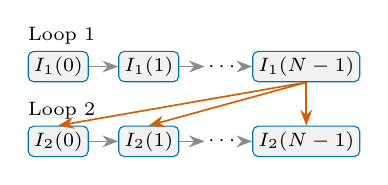
\begin{tikzpicture}[x=1cm,y=1cm,
 instance/.style={draw=origblue,rounded corners=2pt,fill=boxgray,inner sep=2pt,font=\scriptsize},
 carry/.style={->,draw=rulegray},
 dependency/.style={->,draw=staleorange,semithick}]
\node[instance] (a) at (0,0) {$I_1(0)$};
\node[instance] (b) at (1.15,0) {$I_1(1)$};
\node[font=\scriptsize,inner sep=1pt] (gap1) at (2.10,0) {$\cdots$};
\node[instance] (c) at (3.15,0) {$I_1(N-1)$};
\node[instance] (d) at (0,-0.95) {$I_2(0)$};
\node[instance] (e) at (1.15,-0.95) {$I_2(1)$};
\node[font=\scriptsize,inner sep=1pt] (gap2) at (2.10,-0.95) {$\cdots$};
\node[instance] (f) at (3.15,-0.95) {$I_2(N-1)$};
\node[font=\scriptsize,anchor=south west,inner sep=0pt]
  at ([yshift=2pt]a.north west) {Loop 1};
\node[font=\scriptsize,anchor=south west,inner sep=0pt]
  at ([yshift=2pt]d.north west) {Loop 2};
\foreach \s/\t in {a/b,b/gap1,gap1/c,d/e,e/gap2,gap2/f} \draw[carry] (\s) -- (\t);
\foreach \t in {d,e,f} \draw[dependency] (c.south) -- (\t.north);
\end{tikzpicture}
\caption{Schematic of dependent reductions.}
\label{fig:dependent-loops}
\vspace{-6pt}
\end{wrapfigure}

在\emph{依赖归约}中，归约体使用由同一轴上较早归约的最终结果确定的值。
这样的值是它的\emph{上下文}：它沿归约轴保持不变，但只有在较早计算完成后才可用。
\cref{fig:dependent-loops} 中，$I_i(j)$ 表示循环 $i$ 的第 $j$ 次迭代，橙色箭头表示循环之间的依赖。

因此，要将这些归约融合为单遍计算，就需要在最终上下文尚不可用时，先为后续归约积累信息。
为一个输入分块保留的聚合量是\emph{状态分量}，简称\emph{状态}；保留的量共同组成\emph{状态元组}。

\emph{合并}（join）将两个不相交分块的元组组合为其并集对应的元组。
对于使用局部上下文计算的结果，这一操作必须考虑每个分块的上下文变为并集上下文所带来的影响。
由此产生两个相互关联的问题：哪些状态能够保留足够的信息，以及如何推导正确更新这些状态的合并操作。

开发这类算法需要专门经验。
在线归一化、矩累积和分块注意力都需要识别保留量、推导更新，并实现和调优内核~\citep{milakov,chan,pebay,flashattention}。
近期的自动融合方法能够处理平移或缩放局部结果等代数修正~\citep{neptune,redfuser}。
当修正依赖于原有归约结果未保留的聚合信息时，这些规则便不再适用。

\textbf{Our Work.}
本文提出 \sys，\footnote{Greek \emph{hapax}, ``once''.} 通过扩充源归约结果并推导其合并操作，融合依赖张量归约。
我们借鉴为分治并行开发的方法：Farzan 和 Nicolet 综合辅助累加量与合并操作~\citep{farzan17,farzan21}，AutoLifter 则为分治计算综合辅助值和组合函数~\citep{autolifter}。
这些方法引入额外信息，使各分块独立计算的结果能够组合。
\sys 将这一思想用于融合：\emph{辅助状态}补足源结果的上下文修正所需的信息。

\par\medskip
\noindent\begin{minipage}{\linewidth}
\begin{minipage}[t]{0.50\linewidth}
\vspace{0pt}
各分块使用自身的上下文计算状态元组，合并操作再修正并组合这些元组（\cref{fig:dc-fusion}）。
尽管较大分块的元组可能需要多次遍历才能得到，单元素分块的元组只依赖一个输入元素。
在这一构造中，{\bfseries 融合循环}可以视为在一次遍历中依次合并单元素分块的状态元组。
\end{minipage}\hfill
% Shared English vector figure; both prose editions include this source.
% The introducing prose occupies the other half of the enclosing minipage.
\begin{paperdiagram}
\captionsetup{type=figure,skip=4pt}
\centering
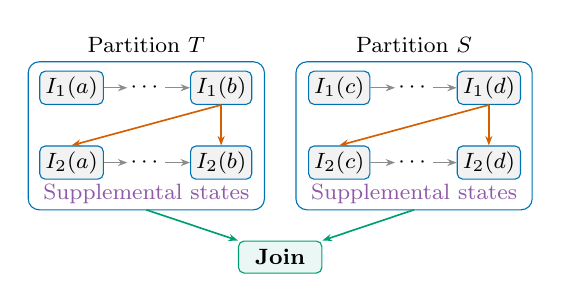
\begin{tikzpicture}[x=1cm,y=1cm,>={Stealth[length=1.2mm,width=0.9mm]},
  label/.style={font=\footnotesize,align=center},
  instance/.style={draw=origblue,rounded corners=2pt,fill=boxgray,
    inner sep=2pt,minimum height=0.32cm,font=\footnotesize},
  continuation/.style={font=\footnotesize,inner sep=1pt},
  part/.style={draw=origblue,rounded corners=4pt},
  joinop/.style={draw=fixgreen,rounded corners=2pt,fill=fixgreen!8,
    inner xsep=6pt,inner ysep=3pt,font=\footnotesize\bfseries},
  carry/.style={->,draw=rulegray},
  dependency/.style={->,draw=staleorange,semithick},
  combine/.style={->,draw=fixgreen,semithick}]

\node[label] at (1.50,0) {Partition $T$};
\node[label] at (4.90,0) {Partition $S$};
\draw[part] (0,-0.22) rectangle (3.00,-2.10);
\draw[part] (3.40,-0.22) rectangle (6.40,-2.10);

% Symbolic endpoints stand for the first and last iterations of each part.
\node[instance] (t1a) at (0.55,-0.55) {$I_1(a)$};
\node[continuation] (t1dots) at (1.50,-0.55) {$\cdots$};
\node[instance] (t1b) at (2.45,-0.55) {$I_1(b)$};
\node[instance] (t2a) at (0.55,-1.50) {$I_2(a)$};
\node[continuation] (t2dots) at (1.50,-1.50) {$\cdots$};
\node[instance] (t2b) at (2.45,-1.50) {$I_2(b)$};
\node[instance] (s1c) at (3.95,-0.55) {$I_1(c)$};
\node[continuation] (s1dots) at (4.90,-0.55) {$\cdots$};
\node[instance] (s1d) at (5.85,-0.55) {$I_1(d)$};
\node[instance] (s2c) at (3.95,-1.50) {$I_2(c)$};
\node[continuation] (s2dots) at (4.90,-1.50) {$\cdots$};
\node[instance] (s2d) at (5.85,-1.50) {$I_2(d)$};
\foreach \a/\dots/\b in {t1a/t1dots/t1b,t2a/t2dots/t2b,s1c/s1dots/s1d,s2c/s2dots/s2d} {
  \draw[carry] (\a.east) -- (\dots.west);
  \draw[carry] (\dots.east) -- (\b.west);
}
% Each part's completed first reduction supplies its second reduction.
\foreach \a/\b in {t1b/t2a,t1b/t2b,s1d/s2c,s1d/s2d}
  \draw[dependency] (\a.south) -- (\b.north);
\node[label,text=auxpurple] at (1.50,-1.90) {Supplemental states};
\node[label,text=auxpurple] at (4.90,-1.90) {Supplemental states};

\node[joinop] (combined) at (3.20,-2.70) {Join};
\draw[combine] (1.50,-2.10) -- (combined.north west);
\draw[combine] (4.90,-2.10) -- (combined.north east);
\end{tikzpicture}
\caption{Partitioned computation.}
\label{fig:dc-fusion}
\end{paperdiagram}

\end{minipage}\par\medskip

为确定哪些信息能够支持这样的合并，\sys 通过代数分析将归约体与其上下文分离。
所得\emph{参考状态}是归约体不读取这些上下文的归约，因而\emph{不依赖上下文}。
它们能够独立合并，并确定所需结果，所以分析成功时便得到一种单遍构造。
其数量给出不随归约长度变化的状态数充分上界。

参考构造提供了一种有效的单遍表示，但执行其展开算术可能破坏源程序的中心化或缩放，引入消去或溢出~\citep{chan,blanchard,boldo_fp}。
这些数值方面的考虑促使我们以源归约在局部上下文下计算的结果作为\emph{维护状态元组}的起点；该元组包含融合程序实际累积的量。
保留这些结果，使源程序中经过中心化或缩放的量能够继续用于上下文修正。
当源结果未保留这些修正所需的足够信息时，辅助状态补足缺失的信息。

\sys 综合辅助状态，使其与源归约结果共同组成能够与参考元组相互转换的维护元组。
对于每个候选维护元组，综合过程构造并验证相应的转换表达式。
通过恢复各分块的参考元组、执行已知的参考合并，再重构并集上的维护元组，即可得到正确的合并操作。
因此，综合只需寻找满足这一转换要求的辅助状态，无需独立搜索合并表达式。

为限制辅助状态的搜索空间，我们根据源归约结果对上下文变化的响应构造候选表达式。
符号化地平移或缩放局部上下文，会引出修正结果所需的聚合系数。
这些系数为语法引导综合提供候选表达式，将搜索限定在对更新有明确作用的量上。
固定的源分量和这些候选共同限制了综合器需要发现的内容。
同样的修正还提供执行公式，在调整局部结果时尽可能复用源程序的中心化和缩放。
以通过恢复得到的合并操作为依据验证这些公式，将数值计算形式与代数正确性论证联系起来。

在实数语义下，所得合并操作计算组合后输入的维护状态元组。
由于合并也适用于任意不相交的非空输入部分，所得归约器允许各分块独立计算后通过归约树组合。
减少遍历为降低数据搬运开销创造了机会；实际性能还取决于状态大小、合并成本和调度。

我们将 \sys 实现为 TVM 张量表达式（TE）的重写~\citep{tvm}。
一个已记录的实现快照在机器学习和科学计算中选取的 \nShowcase 个算子中，为 \nShowFused 个推导出单遍归约器。
本文报告覆盖率、发现的状态和推导开销，并介绍实现中用于比较生成程序与源程序精度的 MPFR 检验方法。
GPU 调度和性能评估仍是后续工作。

\noindent 本文的贡献如下：
\begin{itemize}
\item \textbf{Fusion of dependent-reduction patterns.}
上下文分离识别出一类具有单遍构造的依赖归约链，其中包括消费者归约体超出近期自动融合方法所述代数条件的情形，并界定这一构造所需状态数的充分上界。
\item \textbf{Reference-guided state synthesis and join derivation.}
完整恢复参考表示将综合缩减为状态扩充，使独立搜索合并表达式变得不再必要。
\item \textbf{Source-guided search and numerical formulation.}
源结果及其上下文修正限制辅助状态搜索，同时提供尽可能复用源程序中心化和缩放的执行公式。
\item \textbf{Implementation and evaluation.}
TVM 实现，以及 \nShowcase 个算子上已记录的覆盖率、发现的状态和推导开销结果。
\end{itemize}

\begingroup
\setlength{\intextsep}{2pt}
\captionsetup[lstlisting]{justification=raggedright,singlelinecheck=false}
\reservewrapspace{13\baselineskip}
\section{Motivating Example}
\label{sec:example}

\begin{wrapfigure}{r}{0.32\textwidth}
\begin{lstlisting}[style=pseudocode,caption={Two-pass source program.},label={lst:variance-before}]
$t\gets0$
for $j=0,\ldots,N-1$:
    $t\gets t+x_j$
$\mu\gets t/N$
$ss\gets0$
for $j=0,\ldots,N-1$:
    $ss\gets ss+(x_j-\mu)^2$
return $\;ss/N$
\end{lstlisting}
\end{wrapfigure}
方差展示了融合必须消除的依赖。
对于一行数据 $x_0,\ldots,x_{N-1}$，其中 $N>0$，\cref{lst:variance-before} 中的源程序先计算总和 $t$ 与均值 $\mu=t/N$，再累加中心化平方和 $ss$；方差为 $ss/N$。
只有第一次遍历得到最终均值后，第二次遍历才能开始原有计算。

为将这一依赖转化为合并操作，我们先考察使用局部均值计算的结果。
对于非空分块 $S$，令 $t_S$ 和 $ss_S$ 为源程序在该分块上的归约结果，$\mu_S$ 为该分块的均值。
直接计算这些结果仍需遍历该分块两次。
对于不相交分块 $\pa$ 和 $\pb$，沿用源归约运算（本例为 $\oplus=+$）得到 $ss_\pa\oplus ss_\pb=ss_\pa+ss_\pb$。
它通常不等于并集的中心化平方和，因为两个局部结果使用不同的均值，如 \cref{fig:variance}(a) 所示。
正确的合并操作必须处理均值变为共同均值时带来的变化。

因此，我们首先寻找无需共享均值即可组合的状态。
展开中心化归约，可以显式分离其对 $\mu_S$ 的依赖：
\begin{equation}
\label{eq:variance-reference}
ss_S=\sum_{j\in S}(x_j-\mu_S)^2
=\underbracket{\colorbox{boxgray}{$\displaystyle\sum_{j\in S}x_j^2$}}_{q_S}
 -2\mu_S\underbracket{\colorbox{boxgray}{$\displaystyle\sum_{j\in S}x_j$}}_{t_S}
 +\mu_S^2\underbracket{\colorbox{boxgray}{$\displaystyle\sum_{j\in S}1$}}_{n_S}.
\end{equation}
% Queue the overview with the reference-state discussion.
% Shared English visual; both prose editions include this source.
\par\medskip
\noindent\begin{minipage}{\linewidth}
\captionsetup{type=figure}
\centering
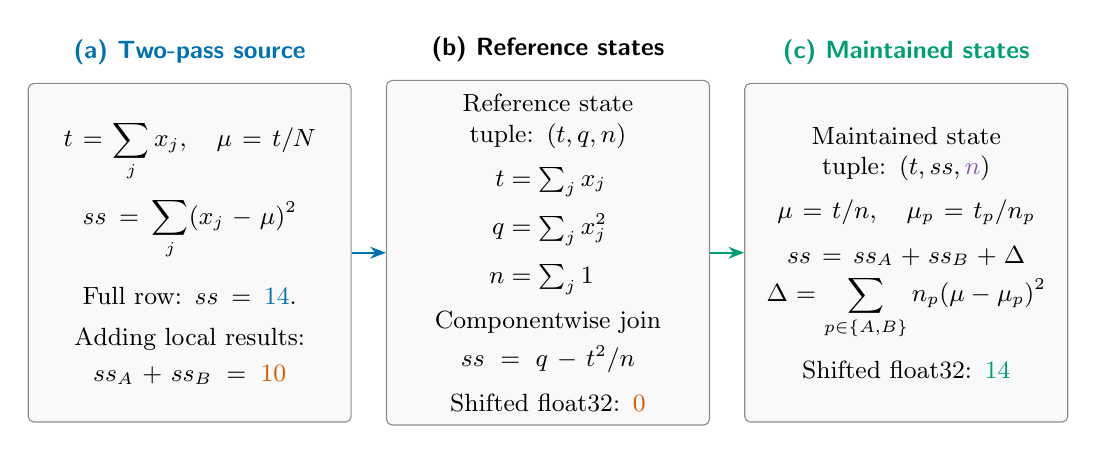
\begin{tikzpicture}[
  summary/.style={draw=rulegray,rounded corners=2pt,fill=boxgray!45,
    text width=3.75cm,minimum height=4.3cm,inner sep=5pt,
    align=center,font=\small},
  heading/.style={font=\sffamily\small\bfseries,anchor=south}]
\node[summary] (source) at (0,0) {
  $\displaystyle t=\sum_j x_j,\quad \mu=t/N$\\[5pt]
  $\displaystyle ss=\sum_j(x_j-\mu)^2$\\[9pt]
  Full row: $ss=\orig{\exTwoPass}$.\\[4pt]
  Adding local results:\\[2pt]
  $ss_\pa+ss_\pb=\stale{\exNaive}$
};
\node[summary] (reference) at (4.55,0) {
  Reference state tuple: $(t,q,n)$\\[5pt]
  $\begin{aligned}
    t&=\textstyle\sum_j x_j\\[2pt]
    q&=\textstyle\sum_j x_j^2\\[2pt]
    n&=\textstyle\sum_j 1
  \end{aligned}$\\[5pt]
  Componentwise join\\[3pt]
  $ss=q-t^2/n$\\[5pt]
  Shifted float32: $\stale{\exTextbookFloat}$
};
\node[summary] (maintained) at (9.1,0) {
  Maintained state tuple: $(t,ss,\aux{n})$\\[5pt]
  $\mu=t/n,\quad \mu_p=t_p/n_p$\\[5pt]
  $ss=ss_\pa+ss_\pb+\Delta$\\[3pt]
  $\displaystyle\Delta=\sum_{p\in\{\pa,\pb\}}n_p(\mu-\mu_p)^2$\\[7pt]
  Shifted float32: $\fix{\exTwoPassFloat}$
};
\node[heading,text=origblue] at ([yshift=3pt]source.north) {(a) Two-pass source};
\node[heading] at ([yshift=3pt]reference.north) {(b) Reference states};
\node[heading,text=fixgreen] at ([yshift=3pt]maintained.north) {(c) Maintained states};
\draw[flow] (source.east) -- (reference.west);
\draw[flow,draw=fixgreen] (reference.east) -- (maintained.west);
\end{tikzpicture}
\caption{Deriving a single-pass variance reducer.
For $\pa=(1,3)$ and $\pb=(2,6)$, adding locally centred results loses the change of mean.
The reference state tuple establishes a three-state bound; the maintained state tuple retains $t$ and $ss$ and adds \aux{$n$} for the correction.
The shifted results report $ss$ after adding $10^4$ to every input.}
\label{fig:variance}
% src: data/illus.json variance_exact and variance_float32
\end{minipage}\par\medskip

\reservewrapspace{10\baselineskip}
\begin{wrapfigure}{r}{0.32\textwidth}
\begin{lstlisting}[style=pseudocode,caption={Single pass with reference states.},label={lst:variance-reference}]
$(t,q,n)\gets(0,0,0)$
for $j=0,\ldots,N-1$:
    $t\gets t+x_j$
    $q\gets q+x_j^2$
    $n\gets n+1$
$ss\gets q-t^2/n$
return $\;ss/n$
\end{lstlisting}
\end{wrapfigure}
高亮的归约均不读取 $\mu_S$：它们分别是平方和 $q_S$、总和 $t_S$ 与计数 $n_S$。
它们构成子图 (b) 中的参考状态元组 $(t_S,q_S,n_S)$。
每个状态都可以通过加法组合，三者共同通过 $\mu_S=t_S/n_S$ 和 $ss_S=q_S-t_S^2/n_S$ 恢复源结果。
这就确立了一个状态数与输入长度无关的充分三状态表示；\cref{lst:variance-reference} 在同一次遍历中累积这些状态，再重构所需结果。

参考表示说明单遍计算在代数上可行，但它重构 $ss$ 时需要对两个可能很大且彼此接近的量做减法。
\cref{fig:variance} 中平移后的 float32 输入展示了由此产生的相消。
为保留中心化计算，\sys 转而从源结果 $(t,ss)$ 出发，分析修正这些结果需要哪些信息。
令 $\mu$ 为并集的均值，$\delta_\pa=\mu-\mu_\pa$ 为 $\pa$ 上的均值变化。
围绕局部均值展开可得
\begin{equation}
\label{eq:variance-rebase}
\sum_{j\in\pa}(x_j-\mu)^2
=ss_\pa-2\delta_\pa\sum_{j\in\pa}(x_j-\mu_\pa)+\delta_\pa^2 n_\pa
=ss_\pa+\delta_\pa^2 n_\pa.
\end{equation}
在实数语义下，由于相对于分块自身均值的偏差之和为零，一次项消失。
剩余修正项以 $n_\pa$ 加权，它表示中心发生变化的元素数量。
源结果 $(t_\pa,ss_\pa)$ 并未保留这一计数。
因此，上下文修正分析将 $n$ 识别为所选表示缺失的信息，\sys 随后将其作为辅助状态进行检验。
在本例中，仅这个系数就足以补全表示：由于 $n_S>0$，维护状态元组 $(t_S,ss_S,n_S)$ 可以恢复 $q_S=ss_S+t_S^2/n_S$，其余参考状态则可直接读取。
状态选择过程验证这一恢复关系后，才接受该元组。

\reservewrapspace{10\baselineskip}
\begin{wrapfigure}{r}{0.32\textwidth}
\begin{lstlisting}[style=pseudocode,caption={Single pass with maintained states.},label={lst:variance-after}]
$\leaf(x)=(x,0,1)$
$a\gets\leaf(x_0)$
for $j=1,\ldots,N-1$:
    $a\gets\Mrg(a,\leaf(x_j))$
$(t,ss,n)\gets a$
return $\;ss/n$
\end{lstlisting}
\end{wrapfigure}
上述上下文修正直接给出 \cref{fig:variance}(c) 中的操作 $\Mrg$：相加总和与计数，并在相加之前将每个局部中心化平方和修正到组合后的均值。
恢复关系提供了规定这一合并操作的另一种方式：恢复各分块的参考元组，相加参考分量，再重构并集的维护元组。
\sys 以这一构造为依据验证中心化公式，将选定状态与正确的合并操作联系起来，而执行时直接计算修正。
对于图示的平移输入的两个分块，这一修正合并与两遍程序的结果一致。

为将这一合并转化为融合，令每个分块恰好包含一个元素。
此时均值为 $x_j$，中心化平方和为零，计数为一，因此初始化函数 $\leaf(x_j)=(x_j,0,1)$ 可直接生成其单元素状态元组。
\Cref{lst:variance-after} 用 $a$ 保存累积元组，从第一个元素初始化，之后每读入一个输入元素，就将这一合并操作应用于相应的单元素状态元组。
这同时消除了分块内部的多次遍历和对全局均值的依赖：输入只读取一次，最终方差为 $ss/n$。

在实数语义下，所得合并恢复了 \citet{chan} 的成对方差公式；逐元素应用时，它在代数上等价于 Welford 更新~\citep{welford}。
同一并集性质还允许通过并行归约树组合。
\endgroup

\reservewrapspace{28\baselineskip}
\section{System Overview}
\label{sec:chains}

\subsection{Derivation Pipeline}

\begin{wrapfigure}{r}{0.48\textwidth}
\centering
% Shared vector source for the paper and standalone diagram.
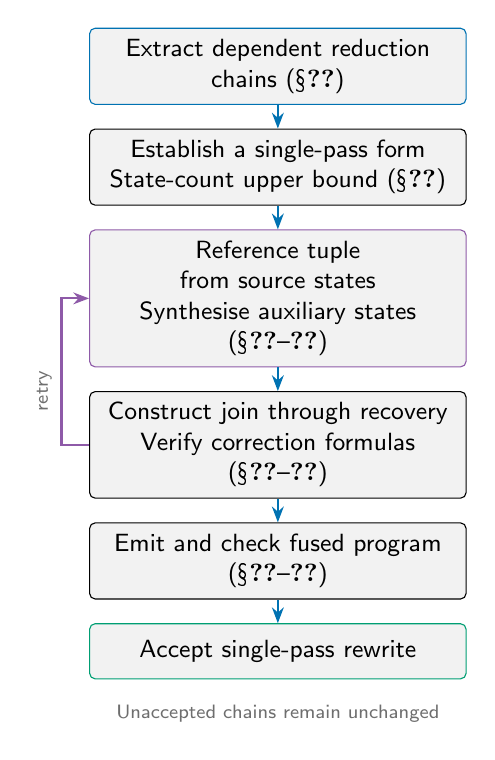
\begin{tikzpicture}[node distance=3mm,
  process/.style={stage,text width=4.5cm,font=\sffamily\small,minimum height=7mm}]
\node[process,draw=origblue] (extract) {Extract dependent reduction\\chains (\S\ref{sec:input-chains})};
\node[process,below=of extract] (judge) {Establish a single-pass form\\State-count upper bound (\S\ref{sec:existence})};
\node[process,below=of judge,draw=auxpurple] (candidate) {Reference tuple from source states\\Synthesise auxiliary states\\(\S\ref{sec:selection}--\ref{sec:synthesis})};
\node[process,below=of candidate] (derive) {Construct join through recovery\\Verify correction formulas\\(\S\ref{sec:recovery}--\ref{sec:rebase})};
\node[process,below=of derive] (check) {Emit and check fused program\\(\S\ref{sec:accuracy}--\ref{sec:impl})};
\node[process,below=of check,draw=fixgreen] (output) {Accept single-pass rewrite};
\foreach \a/\b in {extract/judge,judge/candidate,candidate/derive,derive/check,check/output}
  \draw[flow] (\a) -- (\b);
\draw[flow,draw=auxpurple] (derive.west) -- ++(-0.35,0) |- (candidate.west);
\node[lbl,rotate=90,anchor=south] at ([xshift=-3.5mm]derive.north west) {retry};
\node[lbl,below=2mm of output] {Unaccepted chains remain unchanged};
\end{tikzpicture}

\caption{End-to-end derivation.}
\label{fig:pipeline}
\end{wrapfigure}
\sys 以 TVM Tensor Expressions（TE）表示的程序及其声明的输入域为输入。
如 \cref{fig:pipeline} 所示，它首先提取沿同一轴执行的依赖归约链（\cref{sec:input-chains}），再为各条链推导单遍替代程序。
对于每条提取出的链，代数分析将每个归约的上下文与依赖输入的项分离。
得到的参考状态可以独立合并并确定输出，由此建立状态数上界，作为状态选择的默认限制（\cref{sec:existence}）。

执行其展开公式可能丢失源程序的中心化和缩放，因此选择过程以原有归约结果作为维护状态的起点。
若某个源结果在合法非空分区上无定义，则尝试提取导致定义域问题的上下文、保留其系数，以获得有定义的表示。
为发现缺失的信息，分析器推导将局部上下文替换为更大分区的上下文时，每个保留结果如何变化。
这些修正的系数提供候选辅助状态。
过程首先检查源状态自身，然后检查加入全部可用修正系数后的元组，即重定基闭包。
只有这两个元组都无法在状态数限制内成功时，语法引导合成才搜索这些特征的组合，随后将参考状态也加入搜索。
因此，修正分析可以直接提供所需辅助状态；当这些初始选择不足以满足要求时，合成进一步寻找紧凑的组合（\cref{sec:selection,sec:synthesis}）。

对于每个提出的维护元组，验证过程构造表达式，恢复用于表示其状态及所需输出的完整参考元组，并证明其恒等关系及在合法分区上的有定义性。
由此定义符号形式的合并操作：恢复两个分区的参考状态，分别组合，再将结果表示为维护状态。
验证确立合并后的元组等于并集的状态；证明未成功时，在搜索限制内返回状态选择。
随后，将已验证的合并重写为维护状态上的直接修正，尽可能保留中心化和缩放，以保持源程序的数值行为（\crefrange{sec:recovery}{sec:rebase}）。

后端生成 TE 程序，为每个输入元素计算叶状态元组，合并这些元组，再通过收尾计算产生所需输出。
针对归约器的静态检查与重建程序上的差分数值测量决定是否接受这一浮点实现（\cref{sec:accuracy,sec:impl}）。
若未找到通过验证的构造，或代码生成、数值检查失败，则保留源归约链。


\subsection{Input Reduction Chains}
\label{sec:input-chains}

提取出的链包含沿同一轴执行的归约及其间计算。
\Cref{fig:grammar} 给出了归约体的语言；以下定义说明链内依赖及其在分区上的语义。

\begin{figure}[htbp]
\small
\begin{align*}
f \;::=\;& x \mid \ctx \mid c \mid N
 \mid f + f \mid f - f \mid f \times f \mid f \div f
 \mid \exp f \mid \log f \mid \sqrt{f} \mid f^{k} \mid |f| \mid \max(f,f) \mid \min(f,f)\\
m \;::=\;& \textstyle\bigoplus_{j} f \mid g(\ctx_1,\dots,\ctx_p)
\end{align*}
\caption{Reduction bodies $f$ and chain members $m$. $x$ ranges over the values a chain reads at position $j$ of the axis, $\ctx$ over earlier members, $c\in\R$ over constants, $k\in\mathbb{Z}$, $N$ is the extent of the axis, and $\oplus\in\{\Sigma,\max,\min\}$.}
\label{fig:grammar}
\end{figure}

\begin{definition}[Reduction chain]
\label{def:chain}
固定一个轴 $\Ax=\{0,\dots,N-1\}$；对每个位置 $j\in\Ax$，以元组 $x_j$ 表示归约链在位置 $j$ 从链外张量读取的值。
\emph{归约链}是按生产者先于使用者的顺序排列的成员序列 $m_1,\dots,m_n$。
成员可以是\emph{归约环节} $m=\bigoplus_{j\in\Ax} f_m(x_j,\ctx_m)$，其中 $\oplus\in\{\Sigma,\max,\min\}$；也可以是一个\emph{值} $m=g_m(\ctx_m)$。
\emph{上下文} $\ctx_m$ 是 $m$ 使用不含 $j$ 的索引读取的较早成员，即这些成员的最终值。
只要某个归约环节读取了上下文，就称该链\emph{具有依赖关系}。
\end{definition}

在贯穿全文的方差示例中，最终求和读取均值作为上下文。
\sys 从 TE 程序中提取归约链：TE 归约成为归约环节，链沿 $j$ 读取的逐元素张量则内联到归约体中。
其他轴上的归约，例如注意力中的 $QK^\top$，保留在链外并提供 $x_j$ 中的值。

为了讨论轴的一部分，我们只在该部分上对归约链求值。

\begin{definition}[Partial semantics]
\label{def:partial}
对于非空的 $S\subseteq\Ax$，当每个归约环节仅在 $S$ 上归约、每个上下文取其自身在 $S$ 上的值、作为数值读取的轴长度 $N$ 取 $|S|$ 时，成员 $m$ 的值记为 $m(S)$。
原程序计算的是 $m(\Ax)$。
\end{definition}

声明的输入域约束元素值。
合法分区是满足这些约束的输入的任意非空部分。
即使完整输入的输出有定义，某个原始成员仍可能在这样的分区上无定义；维护状态则必须在每个合法分区上都有定义。
单遍算法必须从逐个分区收集的信息中，在源输出有定义的地方得到 $m(\Ax)$。

\subsection{Single-Pass Reducer Contract}

生成的程序必须从每个元素初始化状态元组，在不重新访问输入的情况下合并这些元组，并恢复所需输出。
以下约定给出每次合并在实数语义下必须保持的关系。

\begin{definition}[Single-pass reducer]
\label{def:reducer}
非空分区上的函数元组 $\st=(\st_1,\dots,\st_k)$ 称为\emph{状态映射}。
固定非归约索引后，每个函数的值均为标量，给定归约器的元组大小 $k$ 固定，不随归约长度 $N$ 增长。
归约链的\emph{单遍归约器}是由叶状态 $\leaf(x_j)=\st(\{j\})$、二元操作 $\Mrg$ 和收尾计算 $\epi$ 构成的元组 $(\leaf,\Mrg,\epi)$，对任意不相交的非空分区 $\pa$ 和 $\pb$，满足
\begin{equation}
\label{eq:invariant}
\Mrg(\st(\pa),\st(\pb))=\st(\pa\dunion\pb),\qquad
\epi(\st(\Ax))=\bigl(m(\Ax)\bigr)_{m\text{ required}}.
\end{equation}
\emph{所需}成员是程序其余部分读取的成员。
\end{definition}

生成的归约从第一个叶状态开始，随后折叠其余叶状态。
没有数值状态代表空分区：执行时跳过空分区，且输入轴必须非空。
\cref{eq:invariant} 中的合并不变量将维护状态元组与原程序联系起来。

\begin{lemma}[Laws from the invariant]
\label{lem:laws}
如果不变量成立，则在两两不相交的非空分区状态上，$\Mrg$ 满足交换律和结合律。
对 $\Ax$ 的任意非空分区划分，以及这些分区上的任意二叉合并树，合并叶状态均得到 $\st(\Ax)$。
从第一个叶状态初始化的串行折叠也具有相同性质。
\end{lemma}

\begin{proof}
$\Mrg(\st(\pa),\st(\pb))=\st(\pa\dunion\pb)=\st(\pb\dunion\pa)=\Mrg(\st(\pb),\st(\pa))$，结合律同样由 $\dunion$ 的结合律推出。
其余结论分别通过对合并树和折叠长度的归纳得到。
\end{proof}

因此，每个非空分区可以独立计算自己的状态元组。
合并树组合这些元组，无需再次遍历各个分区。
这一并行结构来自不变量，而不依赖某个特定调度。

用程序演算的术语来说，$S\mapsto\st(S)$ 是从以 $\dunion$ 为运算的有限非空多重集到以 $\Mrg$ 为运算的状态的同态，即合并与顺序无关的列表同态~\citep{bird87,gibbons96}。
用数据库的术语来说，具有无上下文参考构造的链是一个\emph{代数型}聚合，可由固定数量的\emph{分配型}聚合计算得到~\citep{datacube}。
空分区由控制流处理，不属于代数合并的约定范围。

\paragraph{Problem.}
给定一个依赖归约链，建立单遍归约器的充分条件，构造归约器，证明 \cref{eq:invariant}，并且仅当浮点计算在检查的输入上不引入额外的非有限结果、测得误差相对于原程序保持在规定界限内时接受融合。

\section{A Sufficient Condition for a Single Pass}
\label{sec:existence}

归约环节在每个位置 $j$ 读取上下文，但只有到达轴的末尾才能知道上下文的最终值。
当每个归约环节都能\emph{摆脱}其上下文时，就存在单遍算法：将它重写为上下文与不读取上下文的归约的函数。
本节给出实现这种分离的规则、应用规则的算法，以及由此得到的结论。

\subsection{Freeing a Reduction from Its Contexts}
\label{sec:freeing}

若操作 $\varphi$ 满足 $\varphi(a\oplus b)=\varphi(a)\oplus\varphi(b)$，则称其与归约 $\oplus$ \emph{可交换}。
\Cref{tab:rules} 列出 \sys 能够移到归约外部的操作；在附加条件成立且所有表达式有定义时，每条规则都是 $\R$ 上的恒等式。
求和对加法满足分配律，并允许提取与 $j$ 无关的因子。
最大值归约允许提取加法项、已证明非负的因子或非递减函数。
依赖上下文的项取偶次幂或绝对值时，可以转化为两个极值的较大者。

\begin{table}[t]
\footnotesize
\caption{Operations that commute with a reduction over $j$; $a$, $c$ and $y$ do not depend on $j$. Each rule is an identity under its side condition, which \sys proves syntactically before applying it.}
\label{tab:rules}
\begin{tabular}{@{}llp{0.42\linewidth}@{}}
\toprule
\textbf{Reduction} & \textbf{Rewrite} & \textbf{Side condition}\\
\midrule
$\sum_j$ & $\sum_j (u_j+v_j)=\sum_j u_j+\sum_j v_j$ & none\\
$\sum_j$ & $\sum_j a\,u_j=a\sum_j u_j$, \ $\sum_j e^{u_j+y}=e^{y}\sum_j e^{u_j}$ & none\\
$\max_j$ & $\max_j (u_j+a)=\max_j u_j+a$ & none\\
$\max_j$ & $\max_j c\,u_j=c\max_j u_j$ & $c\ge 0$ proven\\
$\max_j$ & $\max_j h(u_j)=h(\max_j u_j)$ & $h$ non-decreasing on the relevant domain\\
$\max_j$ & $\max_j |u_j|^{2k}=\max(\max_j u_j,\ \max_j -u_j)^{2k}$ & integer $k\ge1$\\
$\min_j$ & dual to $\max_j$ & dual\\
\bottomrule
\end{tabular}
\end{table}

下面的分离将归约体拆为 $r$ 个贡献项。
每个 $g_k$ 包含依赖输入数据的部分，$\varphi_{k,\ctx}$ 则承载该项对上下文的依赖。
重组时将上下文视为固定参数；因此，在尚不知道其值时，就可以先累积所得摘要。

\begin{lemma}[Regrouping]
\label{lem:regroup}
设 $f(x,\ctx)=\bigoplus_{k=1}^{r}\varphi_{k,\ctx}(g_k(x))$，其中所有 $g_k$ 都不读取上下文，且每个 $\varphi_{k,\ctx}$ 都与 $\oplus$ 可交换。
则对任意非空分区 $S$，有 $\bigoplus_{j\in S} f(x_j,\ctx)=\bigoplus_{k=1}^{r}\varphi_{k,\ctx}\bigl(\bigoplus_{j\in S} g_k(x_j)\bigr)$。
\end{lemma}

\begin{proof}
利用 $\oplus$ 的结合律和交换律重排归约，再将每个 $\varphi_{k,\ctx}$ 提取出来。
\end{proof}

所得元组无需知道最终上下文即可计算。上下文仅在从元组重构所需成员时使用。

\subsection{The Judgement}
\label{sec:judge}

参考原子是无上下文归约 $q(S)=\bigoplus_{j\in S}g(x_j)$，由其归约操作及规范化的归约体标识。
归约体允许为常量：$|S|=\sum_{j\in S}1$ 就是以加法为操作、以 $1$ 为归约体的原子。
收集原子前，按照部分语义，将所有作为数值读取的归约轴长度规范化为这一求和。
从求和中提取常量项也可能产生同一个原子。
这两种来源进入同一集合，并通过规范形式相等进行共享；只有所需表达式使用某个原子时，才将其加入集合。

\begingroup
\setlength{\intextsep}{2pt}
\reservewrapspace{16\baselineskip}
\begin{wrapfigure}{r}{0.48\textwidth}
\begin{minipage}{\linewidth}
\begin{algorithm}[H]
\small
\caption{\textsc{Judge}$(\mathit{chain}, \mathit{req})$}
\label{alg:judge}
\KwOut{reference atoms $\mathcal Q$, or failure}
Normalise extent reads in $\mathit{chain}$\;
$W\leftarrow \mathit{req}$;\ $\mathcal Q\leftarrow\emptyset$\;
\While{$W$ not empty}{
  $m\leftarrow$ pop $W$\;
  $e\leftarrow$ free contexts from body of $m$\;
  push unvisited dependencies of $e$ onto $W$\;
  \ForEach{atom $q$ in $e$}{
    \lIf{$q$ reads a context}{\Return \textsc{Stuck}$(m,q)$}
    $\mathcal Q\leftarrow\mathcal Q\cup\{q\}$ (canonical form)\;
  }
}
\Return \textsc{Fusible}$(\mathcal Q)$\;
\end{algorithm}
\end{minipage}
\end{wrapfigure}
\Cref{alg:judge} 访问每个所需成员及其依赖，每个成员只处理一次。
算法将上下文替换为沿归约轴保持不变的符号，通过 \cref{tab:rules} 重写归约体，并将剩余原子收集到 $\mathcal Q$ 中。
仍然读取上下文的原子称为\emph{受阻}：这些规则无法将它与上下文分离。
否则，收集到的原子构成参考状态元组，每个不同的原子对应一个状态。

这一构造给出有限摘要，其分量可以独立合并，其值能够确定所需输出。
它的大小界定了这一构造的状态数；状态选择将该上界用作默认状态数限制。
它也确定了验证所选表示时使用的无上下文量。
这两种作用需要区分：这一构造的存在性并不意味着每种保留原始结果的表示都能满足同一限制。

\finishwrapspace
\endgroup

\begin{theorem}[Existence]
\label{thm:existence}
设 \textsc{Judge} 返回 \textsc{Fusible}$(\mathcal Q)$，其中
\[
\mathcal Q=\{q_1,\dots,q_k\},\qquad
q_i(S)=\bigoplus_{j\in S}^{(i)}g_i(x_j).
\]
如果收集到的归约体在声明的元素域上都有定义，则该链存在至多使用 $|\mathcal Q|$ 个状态的单遍归约器。
其状态元组为 $(q_1(S),\dots,q_k(S))$，合并逐分量进行，收尾计算在源输出的定义域上重构所需输出。
\end{theorem}

\begin{proof}[Proof sketch]
轴长度的规范化保持部分语义；在已证明的附加条件下，每条代数重写在源定义域上都是 $\R$ 上的恒等式。
由 \cref{lem:regroup} 并按生产者顺序归纳可知，在源计算有定义的地方，每个所需成员都具有以收集到的原子表达的重构表达式。
对于每个原子，都有 $q_i(S\dunion T)=q_i(S)\oplus_i q_i(T)$。
因此，该元组可以逐分量合并，其叶子为 $(g_1(x_j),\dots,g_k(x_j))$。
定义域假设保证这些状态在合法非空分区上都有定义；在根节点应用重构表达式，即得到所需输出。
每个原子对应一个坐标，从而得到状态数上界。
\end{proof}

该判定识别能够通过这些规则分离上下文的归约链。
当剩余归约仍依赖某个上下文时，分析停止，不产生构造。
更多恒等式或更强的输入关系可能在这一已识别类别之外进一步建立可归约性。

这一构造是代数参考，不一定是适合实际执行的数值形式。
将上下文从归约体中分离会改变中间量：原本相消的项可能变成很大的独立求和，有界表达式可能变成无界因子的乘积。
保留源归约结果能够保留其中心化和缩放，而辅助状态提供合并所需的信息。
因此，下一步是推导实际维护的表示，并证明它保留了该构造所需的信息。

\section{Synthesising States and Deriving the Reducer}
\label{sec:derivation}

参考构造已经提供一个能够逐分量合并的状态元组，但展开后的分量可能丢失源程序中有利于数值计算的中心化和缩放结构。
我们的任务是寻找另一种表示：保留源归约，发现其部分结果中缺少的信息，并为补充后的元组推导合并操作。
为此，我们将上下文变化的代数分析与辅助状态的语法引导合成结合起来。
构造性的恢复证明将新表示与参考状态元组联系起来，并把已知的合并操作转移到维护状态上。

\subsection{Constructing Candidate Expressions from the Source Reductions}
\label{sec:selection}

令 $A_0(S)$ 为源归约在非空分块 $S$ 上、使用局部上下文求值得到的结果元组。
我们从这些结果出发，是因为其定义可能体现了中心化和缩放等数值计算上的选择。
浮点计算的精度取决于其求值结构，而代数等价的表示可能改变这一结构~\citep{boldo_fp,chan,blanchard}。
保留源定义，使辅助状态合成和合并形式的构造能够继续利用这些数值设计。
如果某个结果在合法分块上没有定义，其定义就不能作为该分块上维护的状态；我们将导致问题的上下文移到归约之外，改为保留所得系数，以修复该表示。
只有已证实的定义域失效才会触发这一定义域修复。
下文中，$A_0$ 均指完成必要修复后的初始维护元组。
我们展开所得 $A_0$ 及所需输出，构造不依赖上下文的参考状态元组 $B(S)$，并得到已知映射 $G_0$，使得 $A_0(S)=G_0(B(S))$。
这一构造独立于 \cref{sec:existence} 中的初始参考集合 $\mathcal Q$：$B$ 可能包含保留源结果所需、但不在 $\mathcal Q$ 中的分量。
$B$ 的分量能够独立合并，并确定所需输出。
这些分量在合成辅助状态之前就已固定：每个新状态都必须是这些分量及固定程序参数的有定义函数。

辅助状态应当提供在上下文变化时修正部分结果所需的信息。
我们通过符号方式将局部上下文替换为平移或缩放后的上下文，再应用参考构造中的代数规则，发现这样的量。
对于由求和归约定义的状态 $r$，在规则的附加条件成立时，成功的展开具有如下形式
\begin{equation}
\label{eq:features}
r(S;\kappa')=\sum_{\ell}\alpha_\ell(\delta,\rho)\,e_\ell(S;\kappa_S),
\end{equation}
其中 $\kappa_S$ 是局部上下文，$\kappa'$ 是目标上下文，$\delta,\rho$ 描述两者之间的加性或乘性变化。
因子 $\alpha_\ell$ 依赖这些变化；系数 $e_\ell$ 则是使用局部上下文求值的聚合量。
分析器尝试平移和缩放修正，优先选择将原状态保留为一个系数的分解，其次选择系数较少的分解。
当原状态是其中一个系数时，其余系数就指出修正所需的信息。
如果一个和分解为具有不同修正因子的贡献项，则将其中可以分别调整的组成项作为候选表达式。
对于极值，对应的单调性和上下文提取规则会暴露可用的修正系数。

可用的修正系数和可以分别调整的组成项构成候选表达式集合 $E_{\mathrm{pre}}$。
每个候选表达式都有两种形式：用 $B$ 表达的定义用于推理，保留局部上下文的结构化归约表达式用于生成代码。
我们排除规范化后成为数值常量（包括零）的表达式，以及重复表达式和 $A_0$ 中已有的表达式；比较时忽略非零有理数缩放。
如果表达式依赖 $B$ 之外的分量，或无法证明其有定义，我们也将其丢弃。
元组 $K$ 只包含保留下来的系数候选；通过拆分求和得到的候选，以及之后为合成加入的参考分量，都不进入 $K$。
因此，每个保留的候选表达式都是参考状态元组的已知函数。
当某个修正系数为 $\sum_{j\in S}1$ 时，计数就通过相同机制进入。
如果参考展开暴露了计数，它就可以和 $B$ 的其他分量一起参与搜索。
算法没有单独的计数选择规则。

\subsection{Synthesising Auxiliary States}
\label{sec:synthesis}

这些候选表达式描述了有用的量，但逐个选取它们未必能得到紧凑而充分的状态元组。
因此，我们合成辅助状态元组 $C=(c_1,\ldots,c_w)$，并维护 $A=(A_0,C)$。
对于候选表达式集合 $E$，每个辅助状态都是以下有限语法中的表达式
\[
\begin{aligned}
\mathcal E_1&::=e\quad(e\in E),\\
\mathcal E_\ell&::=\mathcal E_{\ell-1}
 \mid\mathcal E_{\ell-1}+\mathcal E_1
 \mid\mathcal E_{\ell-1}-\mathcal E_1\qquad(2\le\ell\le d).
\end{aligned}
\]
默认深度 $d=3$ 允许候选表达式的带符号组合，其中候选表达式总共出现至多三次。
候选表达式本身可以是 $B$ 的非线性函数，因此该语法组合的是代数分析已经发现的量，而不要求求解器重新发现其内部的乘法、除法或中心化结构。
每个选中候选表达式的结构形式也随组合一起保留。

合成规约要求补充后的元组能够区分所有可能代表不同部分计算的参考状态元组。
令 $\mathcal R$ 为可达元组的保守过近似，由定义域和有限求和事实约束。
在固定程序参数下，提交给 cvc5 的条件为
\begin{equation}
\label{eq:synthesis}
\forall B_1,B_2\in\mathcal R:\quad
\bigl(G_0(B_1)=G_0(B_2)\ \land\ C(B_1)=C(B_2)\bigr)
\ \Longrightarrow\ B_1=B_2.
\end{equation}
仅有初始状态元组相等，仍可能掩盖合并所需的信息；辅助状态必须能够区分这些情况。
这样就明确了恢复的目标，而不是只检查最终输出是否恰好相等。

\noindent\begin{minipage}{\linewidth}
\begin{minipage}[t]{0.50\linewidth}
\vspace{0pt}
\Cref{alg:select} 分阶段组织搜索。
它首先检查初始元组 $A_0$ 本身，再检查向 $A_0$ 加入保留下来的修正系数 $K$ 后的元组。
如果两者都未成功，原生 SyGuS 先使用 $E_{\mathrm{pre}}$，再使用 $E_{\mathrm{mix}}=E_{\mathrm{pre}}\cup\{B_i\mid1\le i\le|B|\}$。
第一阶段优先考虑保留源结构的修正量；第二阶段加入这些修正量可能遗漏的参考信息。
求解器搜索候选表达式的组合，而不只是候选表达式集合的子集。

每个提案都必须通过独立的构造性检查，记为 \textsc{Verify}：构造恢复映射，证明其恒等关系和定义域，再推导并验证完整归约器。
检查失败后，继续请求原生求解器的下一个解。
如果带量词的合成返回未知，原生语法枚举仍可向同一个检查器提供提案。
这类提案只能凭借构造性证明被接受，而不能凭借未知的合成结果。
\end{minipage}\hfill
\begin{paperdiagram}
\begin{minipage}{\linewidth}
\begin{algorithm}[H]
\small
\SetInd{0.5em}{0.7em}
\caption{\textsc{Select}$(\mathit{chain},b_{\max})$}
\label{alg:select}
$A_0\leftarrow$ source states; repair domain defects\;
$(B,G_0)\leftarrow$ expand $A_0$ and outputs\;
$E_{\mathrm{pre}}\leftarrow$ defined candidate expressions over $B$\;
$K\leftarrow$ correction coefficients in $E_{\mathrm{pre}}$\;
\ForEach{$A\in\{A_0,(A_0,K)\}$ fitting $b_{\max}$}{
\lIf{\textsc{Verify}$(A,B)$ succeeds}{\Return reducer}
}
\ForEach{$E\in[E_{\mathrm{pre}},E_{\mathrm{mix}}]$}{
\ForEach{width $1\le w\le b_{\max}-|A_0|$}{
Propose $C\in\mathcal E_d^{\,w}$ using \eqref{eq:synthesis}\;
On unknown: native enumeration\;
\While{proposals and resources remain}{
\lIf{\textsc{Verify}$((A_0,C),B)$ succeeds}{\Return reducer}
Request next native proposal\;
}
}}
\Return search failure\;
\end{algorithm}
\end{minipage}
\end{paperdiagram}
\end{minipage}\par\medskip

参考构造的状态数上界为 $b_{\mathrm{ref}}=|\mathcal Q|$；我们将其作为维护元组的默认限制 $b_{\max}$。
这一选择并不约束所有保留有定义源结果的表示的大小。
如果 $A_0$ 和 $B$ 均有定义，加入 $B$ 的全部分量总能通过投影实现恢复，状态数至多为 $|A_0|+|B|$。
这确立了一种充分构造，证明见附录 A；它并不保证紧凑元组能够满足 $b_{\max}$，也不保证有界合成能找到这样的元组。
搜索采用受限语法和独立证明过程，不声称所得表示最小。

\subsection{Constructing and Verifying Recovery}
\label{sec:atoms}
\label{sec:recovery}

对于候选 $A=(A_0,C)$，选中表达式的定义给出 $G(B)=(G_0(B),C(B))$，因此 $A(S)=G(B(S))$。
单射性是信息层面的要求；生成归约器还需要可执行的恢复映射 $H$，满足
\begin{equation}
\label{eq:recovery}
H(G(B(S)))=B(S).
\end{equation}
该恒等式在合法非空分块产生的元组上成立，也给出相应维护表示上的 $G(H(A(S)))=A(S)$。
恢复从维护元组重构参考状态分量。
\Cref{fig:recovery-square} 用贯穿全文的方差示例展示辅助状态构造、恢复及合并推导。
% Both panels and their common caption form one full-width figure.
% Shared unchanged by the English and Chinese prose editions.
\par\medskip
\noindent\begin{minipage}{\linewidth}
\captionsetup{type=figure}
\centering
\begin{minipage}[t]{0.48\linewidth}
\vspace{0pt}
\centering
{\small\sffamily\bfseries (a) State relations}\par\medskip
% Shared vector source for the English and Chinese prose editions.
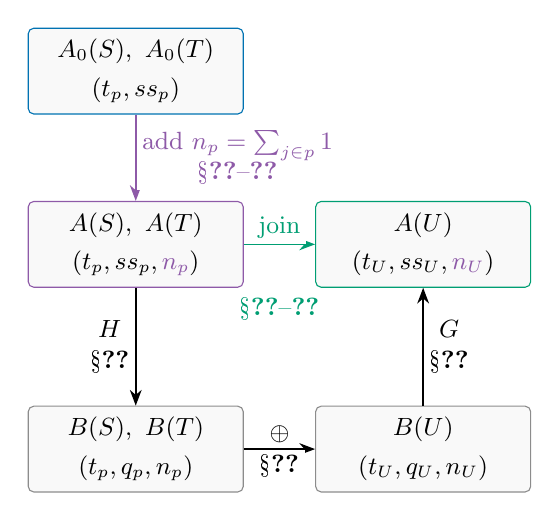
\begin{tikzpicture}[
  summary/.style={draw=rulegray,rounded corners=2pt,fill=boxgray!45,
    text width=2.45cm,minimum height=1.05cm,inner sep=4pt,
    align=center,font=\small},
  arrow/.style={-{Stealth[length=2mm]},semithick},
  label/.style={font=\small,fill=white,inner sep=2pt,align=center}]
\node[summary,draw=origblue] (original) at (0,2.2)
  {$A_0(S),\ A_0(T)$\\[3pt]$(t_p,ss_p)$};
\node[summary,draw=auxpurple] (maintained) at (0,0)
  {$A(S),\ A(T)$\\[3pt]$(t_p,ss_p,\aux{n_p})$};
\node[summary,draw=fixgreen] (merged) at (3.65,0)
  {$A(U)$\\[3pt]$(t_U,ss_U,\aux{n_U})$};
\node[summary] (reference) at (0,-2.6)
  {$B(S),\ B(T)$\\[3pt]$(t_p,q_p,n_p)$};
\node[summary] (combined) at (3.65,-2.6)
  {$B(U)$\\[3pt]$(t_U,q_U,n_U)$};
\draw[arrow,draw=auxpurple] (original) --
  node[label,right,text=auxpurple] {add $n_p=\sum_{j\in p}1$\\\S\ref{sec:selection}--\ref{sec:synthesis}} (maintained);
\draw[arrow,draw=fixgreen] (maintained) --
  node[label,above,text=fixgreen] {$\Mrg$}
  node[label,below=6mm,text=fixgreen] {\S\ref{sec:correctness}--\ref{sec:rebase}} (merged);
\draw[arrow] (maintained) -- node[label,left] {$H$\\\S\ref{sec:recovery}} (reference);
\draw[arrow] (reference) -- node[label,above] {$\oplus$}
  node[label,below] {\S\ref{sec:correctness}} (combined);
\draw[arrow] (combined) -- node[label,right] {$G$\\\S\ref{sec:atoms}} (merged);
\end{tikzpicture}

\end{minipage}\hfill
\begin{minipage}[t]{0.48\linewidth}
\vspace{0pt}
\small
\centerline{\sffamily\bfseries (b) Derivation}
\medskip
On each part, let $t=\sum_jx_j$, $q=\sum_jx_j^2$ and $n=\sum_j1$.
Expanding the source definition gives
\[
G(t,q,n)=(t,q-t^2/n,n).
\]
From $(t,ss)$, recovery leaves $q=ss+t^2/n$ dependent on the unknown $n$.
Adding $n$ gives the complete recovery
\[
H(t,ss,n)=(t,ss+t^2/n,n).
\]
Since $n>0$, both maps are defined and $H\circ G=\mathrm{id}$.
The reference join $\oplus$ adds coordinates.
The upper arrow follows by composition:
\[
\Mrg(a,b)=G\bigl(H(a)\oplus H(b)\bigr).
\]
With $t_U=t_S+t_T$ and $n_U=n_S+n_T$, rewriting yields the centred form
\[
\begin{aligned}
ss_U={}&ss_S+ss_T\\
&+\frac{n_Sn_T}{n_U}
  \left(\frac{t_S}{n_S}-\frac{t_T}{n_T}\right)^2.
\end{aligned}
\]
The emitted join evaluates this correction without materialising $q$.
\end{minipage}
\caption{Variance: auxiliary states, recovery and join derivation.
Here $p\in\{S,T\}$ and $U=S\dunion T$ for disjoint non-empty parts.
Arrow annotations identify the subsections that develop each step:
feature construction and synthesis (\S\ref{sec:selection}--\ref{sec:synthesis}), information equivalence (\S\ref{sec:recovery}),
join derivation (\S\ref{sec:correctness}), and numerical formulation (\S\ref{sec:rebase}).}
\label{fig:recovery-square}
\end{minipage}\par\medskip


恢复过程从定义 $A$ 的方程中消去参考状态分量。
它代入已知表达式，并利用支持的代数规则解出一个剩余分量。
中间表达式可以依赖其他未知分量；接受之前，必须通过反复代入消除所有这类依赖。
$B$ 的每个分量最终都必须用维护状态和固定参数表示。
这一过程单独构造 $H$，与搜索 $C$ 的 SyGuS 合成相区分。

每次引入除法都需要定义域证明。
对于可能为零的除数，只有证明相应的待恢复分量在零分支上也为零，才能在该分支返回零。
有限求和规律能够独立于分块长度证明此类蕴含：非负项之和为零意味着每一项都为零。
符号规范化和 SymPy 证明恒等关系，Z3 检查定义域及带条件的蕴含关系。
惰性条件表达式确保不执行未选中分支中的除法。
这些检查说明，合成出的单射映射仍只是提案，而非可以立即执行的归约器。

\subsection{Deriving the Join and Proving Correctness}
\label{sec:correctness}

参考状态分量是不依赖上下文的归约，因此可以通过操作 $\oplus$ 逐分量组合。
对于不相交的非空分块 $S,T$，它们满足 $B(S\dunion T)=B(S)\oplus B(T)$。
建立恢复关系后，合并先恢复两个参考状态元组，组合它们，再将结果表达为维护状态元组：
\begin{equation}
\label{eq:merge}
\Mrg(a,b)=G\bigl(H(a)\oplus H(b)\bigr).
\end{equation}
令 $F$ 将所需输出表示为参考状态元组的函数。
初始化函数 $\leaf(x_j)=A(\{j\})$ 为每个元素生成单元素状态元组。
在源输出的定义域上，输出函数为 $\epi(a)=F(H(a))$；已经保留在 $A$ 中的输出可以直接读取自己的分量。
这些等式规定归约器，而不依赖最终采用的求值顺序。

\begin{theorem}[Correctness over $\R$]
\label{thm:correct}
设 $A=G\circ B$，且 $H\circ G$ 在可达参考状态元组上为恒等映射。
假设初始化对每个合法元素有定义，恢复和合并操作在合法非空分块上有定义，输出函数在源输出有定义的地方也有定义。
则对于任意由非空分块组成的划分及其上的任意二叉合并树，推导出的归约器均计算出源程序的输出。
\end{theorem}
\begin{proof}
对于两个不相交的非空分块，
\[
\begin{aligned}
\Mrg(A(S),A(T))
 &=G\bigl(H(G(B(S)))\oplus H(G(B(T)))\bigr)\\
 &=G\bigl(B(S)\oplus B(T)\bigr)\\
 &=G(B(S\dunion T))=A(S\dunion T).
\end{aligned}
\]
第一个等号代入状态定义；第二个等号使用恢复关系；第三个等号使用逐分量聚合。
因此，每个内部节点计算的都是其后代叶子对应的维护元组。
对树归纳可得根节点的元组，应用 $F\circ H$ 则重构所需输出。
定义域假设确保每个执行的操作都有对应的值。
\end{proof}

不相交分块的并集运算蕴含可达状态上的结合律和交换律。
因此，每个分块可以独立处理，再通过归约树组合，从而得到分治并行结构。
执行时，每个活动分块从自己的第一个元素初始化，并跳过空分块。
证明确立的是包含辅助状态在内的整个元组的结果，而不仅是最终输出。

\subsection{Numerical Formulation of the Join}
\label{sec:rebase}

所选表示的数值优势取决于合并操作的实际求值方式。
即使整体计算的条件良好，等价的计算分解也可能引入会放大误差的中间子问题~\citep{higham_decomposition}。
具体而言，直接执行 $G(H(a)\oplus H(b))$ 可能先重构展开后的参考分量，再从这些分量恢复维护的量。
我们将这一组合重写为直接从维护状态及其局部上下文计算的修正，尽可能避免这些中间重构。
这种数值重写选择合并的求值方式，与修复无定义的源状态及构造候选表达式是不同的操作。
源定义指导数值形式的选择；参考状态元组的恢复则提供推导和验证所需的信息。
在 \cref{fig:recovery-square} 的方差推导中，这一组合变成基于局部均值之差的修正，无需实际构造原始平方和。
中心矩合并和在线 softmax 也通过这种方式，对部分结果重新中心化或缩放~\citep{pebay,milakov}。
生成公式需要与组合形式的合并进行等价性验证，并检查其执行分支的定义域。
\begin{theorem}[Correctness of the emitted join]
\label{thm:printed}
如果生成的合并在可达状态上经验证与组合形式的合并相等，且执行的分支均有定义，那么它满足相同的合并不变量。
\end{theorem}
\begin{proof}
代入已经验证的等式，即保留上述证明中的不变量。
\end{proof}
保留源状态并用上下文修正表达合并，指导其数值形式的选择；代数证明确立其在实数上的正确性。
随后对生成程序进行静态检查，并与源程序比较精度，以判断其浮点行为是否可接受。

\section{Keeping the Accuracy of the Original Program}
\label{sec:accuracy}

推导出的归约器现在具有经验证的合并操作和选定的数值形式。
它在浮点数上执行，求值顺序和中间量与源程序不同~\citep{higham,goldberg}。
为判断这一形式是否可接受，\sys 将生成表达式的静态检查与相对于原程序的差分测量结合起来。
测量采用以下接受判据。

\begin{definition}[Accuracy acceptance]
\label{def:gate}
对于结果 $\hat y$，以原程序在 float64 中的计算结果 $y$ 为参考，定义误差为 $\max|\hat y-y|/\max|y|$；若 $\hat y$ 的任一值非有限，则误差为 $\infty$。
如果对一组输入中的每个输入，融合后的程序仅在原程序产生非有限值的地方产生非有限值，且误差不超过 $100\max(\mathit{err}_{\mathrm{orig}},\mathit{err}_{\mathrm{inh}})+64u$，就称其在这组输入上\emph{通过精度检查}。其中 $\mathit{err}_{\mathrm{inh}}$ 是通过输入扰动得到的经验敏感度估计，$u=2^{-23}$。
\end{definition}

这一界限相对于原程序，而不是精确答案：融合程序允许的精度损失，以原程序或问题条件性所导致的损失为基准，并允许一个常数因子。
检查仅施加于采样输入，因此提供的是证据，而非保证。

\subsection{Static Checks on the Emitted Join}
\label{sec:hazards}
\label{sec:static}

单遍计算同时改变求值顺序和中间量。
并行归约必然涉及运算重结合，而展开为原点矩可能引入相消，移除缩放则可能导致溢出。
另一个风险是除以上下文：该上下文在完整输入上非零，却可能在某个真子分区上为零。
这些风险促使我们在合并允许的情况下，保留源程序的中心化和缩放表示。

\textbf{Proven guarantees.}
随后，\sys 检查所推导合并的两个性质。
只有原程序具有某个性质时，才要求候选也具有该性质。

\begin{proposition}[Bounded exponents]
\label{prop:exp}
合并中每个 $\exp$ 的自变量都不超过 8：每个正项都被同一轴上减去的最大值，或运行中的最大值状态所抵消。
\end{proposition}

\begin{proposition}[Positive divisors]
\label{prop:div}
沿从第一个叶状态初始化的串行折叠，本条件所检查的每个实际执行的除数和对数自变量均为正。
分析结合了符号格 $\{\text{any},\geq0,>0\}$ 上的最大不动点，以及分支条件下的 SMT 蕴含关系。
\end{proposition}

\textbf{Where the join departs from the program.}
程序自身的计算并不总能保留。
当证明某个源归约结果在合法分区上无定义时，\textsc{Select} 将导致问题的上下文移出归约，并将所得系数保留为状态，以修复该定义。
% src: data/fused_ops.json actions; reducer/states.py and reducer/smt.py
即使合并只对原程序状态进行上下文重基，它仍是一个更新公式；当数据偏移相对于其离散程度很大时，更新公式可能比两遍算法损失更多精度，差异可达到问题条件数的量级~\citep{chan}。
这些情况下没有舍入误差证明，只能由下述验收检查决定是否接受。

\subsection{Acceptance Measurements and Their Limits}
上述证明并不判定舍入误差。
因此，\sys 在接受融合之前，会将融合后的程序与原程序进行比较。
系统从五类输入族采样：中心化输入、平移 $10^4$ 的输入、大离散度输入，以及接近溢出和下溢阈值的输入；以原程序的 float64 求值为参考，分别计算两个程序，并在每类输入上检查 \cref{def:gate}。
补充材料的附录 E 详细说明了输入族和测量方法。


\label{sec:accuracy-limits}

\Cref{tab:assurance} 区分了 \sys 所证明的性质与仅在样本上检查的性质。
验收检查是对五类输入族的差分测试，而非证明；没有采样到的输入不在其覆盖范围内，例如声明为正的定义域之外、恰好为零的权重。
执行约定排除了空分区参与合并。
并行实现必须用各自的第一个叶状态初始化每个活动分区，并跳过非活动分区，而不能注入数值单位元。
这是对降层实现的要求，而非精度检查所建立的浮点性质。

\begin{table}[t]
\caption{What each step establishes. \tagP: proven; \tagS: checked on samples; ---: not established.}
\label{tab:assurance}
\footnotesize
\begin{tabular}{@{}lp{0.62\linewidth}l@{}}
\toprule
\textbf{Step} & \textbf{Property} & \\
\midrule
Judgement (\cref{alg:judge}) & defined reference atoms give a single pass with at most $|\mathcal Q|$ states & \tagP\\
Selection (\cref{alg:select}) & complete recovery and defined states on legal non-empty parts & \tagP\\
Join & invariant and leaves (\cref{thm:correct,thm:printed}) & \tagP\\
Join & bounded exponents, positive divisors on the serial fold (\cref{prop:exp,prop:div}) & \tagP\\
Rebuilt program & agrees with the original in float64 on three small shapes & \tagS\\
Rebuilt program & passes the accuracy check (\cref{def:gate}) on five input families & \tagS\\
Rebuilt program & a bound on its floating-point error for every input & ---\\
\bottomrule
\end{tabular}
\end{table}

\section{Implementation}
\label{sec:impl}

\sys 是建立在 TVM 张量表达式之上的 Python 包，约含 \nLoC{} 行非空代码，\nTestFiles 个文件中共有 \nTests 项测试。
% src: gen/stats.tex nLoC, nTests, nTestFiles (counted by scripts/gen_tex.py; tests from data/pytest.log)
入口 \code{fuse(outputs, inputs)} 重写输出所依赖的每条归约链，返回重写后的 TE 及每条链的报告；\code{judge(outputs)} 仅执行判定。
前端从 TE 中读取归约链，将归约体转换为符号形式，使用哈希共享项，并通过 \cref{tab:rules} 的重写保持规范形式。
判定、选择、推导和证明均在这一形式上进行；SymPy 处理规范化未能解决的恒等式。
内部用紧凑节点表示归约域的基数，其含义就是归约体为常量的求和；实现通过单独标志报告它，这等价于将该原子纳入参考集合。
Z3 在可达状态的抽象上检查源定义域、带守卫的恢复定义域和多项式恢复的唯一性。
求解器返回未知时拒绝该证明义务；它不会被视为证明，也不会成为替换有定义源结果的依据。
后端将每个合并打印为 TE 表达式，为每条链生成一个 \commreducer，以第一个叶子初始化并归约其余叶子，添加逐元素收尾计算，然后重建下游张量以读取新状态。
未融合的链保持原样，报告说明原因。


原生 cvc5 SyGuS~\citep{cvc5} 搜索辅助状态，并负责候选枚举及内部细化。
在每个语法阶段，实现先尝试允许的最大辅助状态数，再按递增顺序尝试更少的状态数。
搜索至多考虑 256 个提案，每个辅助状态最多包含三个特征项，并在各语法阶段和状态数选择之间共享 20 秒的合成时限。
语义合成调用的时限为 1500\,ms；已经开始的独立证明可能在总体时限之后完成。
如果合成返回未知，cvc5 的原生语法枚举器可以提供提案，交由独立验证。
对于多项式元组，该检查器还要求双副本唯一性查询得到证明，以补充构造性恢复证明。
源状态修复至多进行 64 轮，每个 Z3 查询的时限为 1500\,ms。
数值检查拒绝候选时保留源归约链，不会重新启动状态合成。

要求的定义域性质涉及每个合法非空输入分区。
为决定是否可以替换原始归约结果，当前实现将单元素分区代入源定义，检查是否存在使其无定义的合法元素值，从而寻找具体见证。
这样的单元素分区本身就是合法分区，因此足以反驳定义域性质。
见证搜索仅限于这一情形，不检验任意分区大小。
未解决的恢复等式或抽象坐标域中的可满足模型，都不能确立源定义域失效。
这一区分使有定义的原始结果得到保留，同时允许在部分语义确实失效时进行修复。

前端接受上述算术语言、单个归约轴，以及求和、最大值和最小值归约器。
不支持的控制流、索引或函数使该链保持原样。
代数分析使用列出的重写规则，而不使用任意依赖输入的恒等式。
符号重写、SymPy 恒等式、有限求和事实以及将定义域义务转换为 Z3 查询的过程构成证明基础；超越运算通过支持的恒等式和保守符号事实处理。
超时及不支持的证明义务均导致拒绝。


输出是普通 TE。
\code{te.create\_function} 将其降低为 TIRx 中的函数；TIRx 是我们使用的 TVM 版本以独立包 \code{tvm\_tirx} 提供的张量 IR，TVM 再通过 LLVM 将其编译到 CPU。
\sys 使用这一路径在重建后的程序上执行 float64 一致性检查和精度门控。
\sys 不执行调度：评估考察哪些程序能够融合、推导和证明了什么，以及结果的精度。

\textbf{GPU lowering.}\par
\label{sec:gpu}

\ifsubmit\else
\placeholder{GPU code generation through TIRx. 待结合后端补充：如何调度推导出的 \commreducer（线程、warp、block 层级，以及沿归约轴的 split-K）；如何在单遍计算内部逐块计算 $QK^\top$ 等边界生产者；以及如何跳过空分区并初始化每个活动分区（\cref{sec:accuracy-limits}）。}
\fi
推导出的归约器是满足结合律和交换律的元组合并，这正是 GPU 树形归约及跨线程块划分归约轴所需的形式。
将它转化为高效内核是 TVM 调度和 TIRx 分块原语的工作，不属于本文范围。
其中有两个针对推导合并的具体问题需要处理。
首先，链沿归约轴读取的生产者，例如注意力分数，仍被物化；需要像手工实现的 FlashAttention 一样，在融合循环内分块计算它们。
其次，每个活跃分区必须从自己的第一个叶子初始化，并跳过非活跃分区。TE 初始化表达式不是通用归约调度可以复制的中性元。

\section{Evaluation}
\label{sec:eval}

我们评估四个问题。
\textbf{RQ1}：\sys 能否融合实际使用的依赖归约？
\textbf{RQ2}：它引入了哪些状态？
\textbf{RQ3}：推导和证明的开销是多少？
\textbf{RQ4}：相对于源程序和直接执行参考状态的程序，维护状态如何影响数值精度？

下文的覆盖范围、所选状态和推导耗时记录于合成版本 \code{6c46fb1b02}。
\placeholder{使用更新后的数值检验协议，重新测量依赖验收判定的结果、MPFR 精度和完整融合耗时。}


我们从应用中选取了 \nShowcase 个算子，其归约之间具有不同的依赖方式（\cref{tab:showcase}）。
应用包括语言模型（注意力、交叉熵、LayerNorm 及其反向计算）、强化学习与多模态预训练、最优传输、统计计算、无线通信、数值线性代数和统计物理。
多数算子已有库中的手工单遍实现；表格列出已记录的实现，条目缺失不表示不存在相应实现。
每个算子均按其定义写为 TE，并提供手写单遍实现用于比较。
它们来自包含 \nRegistry 个算子的注册表，其中许多是这些算子的变体；补充材料附录 B 报告注册表中已融合的算子，附录 C 列出其他融合结果及失败原因。


所有程序采用 float32 和符号维度。
已记录的实验使用 Python \pythonVersion、SymPy \sympyVersion、Z3 \zThreeVersion 和 cvc5 \cvcFiveVersion。
所报告的推导耗时是在 Intel Xeon Platinum 8468H 上预热后运行五次的中位数。
% src: data/fused_ops.json meta (cpu, extent, seed, offset); data/proofs_timing.json meta.repeats

\begin{table}[t]
\caption{Recorded coverage and state discovery. ``Hand-fused in'' lists identified library implementations; a dash means none is recorded. Passes count traversals of the fused axes. Derived components are absent from the source reduction results, including replacements after domain repair. Selection route reports the initial tuple alone, augmentation with all correction coefficients, or synthesis (including independently verified enumeration).}
\label{tab:showcase}
\footnotesize
\setlength{\tabcolsep}{3pt}
\begin{tabular}{@{}>{\raggedright\arraybackslash}p{0.24\linewidth}>{\raggedright\arraybackslash}p{0.28\linewidth}ccc>{\raggedright\arraybackslash}p{0.12\linewidth}@{}}
\toprule
\textbf{Operator} & \textbf{Hand-fused in} & \textbf{Passes} & \textbf{States} & \shortstack{\textbf{Derived}\\\textbf{components}} & \shortstack[l]{\textbf{Selection}\\\textbf{route}}\\
\midrule
\tabShowcaseRows
\bottomrule
\end{tabular}
\end{table}

\subsection{Fusion Coverage and State Selection}
\label{sec:eval-coverage}

在所记录的版本中，\sys 融合了 \nShowcase 个算子中的 \nShowFused 个。
这些算子的 \showChains 条链在融合前共遍历各自归约轴 \showPassesBefore 次，融合后为 \showPassesAfter 次，每条链一次；对比损失和 Sinkhorn 迭代均有两条链，分别沿行和列归约。
手写单遍实现具有相同的遍历次数。
推导出的归约器包括在线 softmax、FlashAttention 的归一化归约器，以及 LayerNorm 和 Pearson 相关系数中的成对中心矩合并~\citep{chan}。
热容通过加权多项式读取均值，超出了已有融合编译器所述条件（\cref{thm:containment}）。


\paragraph{Derived representation.}
\label{sec:eval-states}

这 \showChains 个归约器共有 \showStates 个状态，其中 \showDerived 个是原程序未计算的量，分布于 \showDerivedOps 个算子中（\cref{tab:showcase}）。
\showOriginalOps 个算子仅凭初始元组即可通过验证，\showRebaseOps 个补充全部修正系数，\showSygusOps 个使用原生合成。
对于 PAPR，源程序保留总和、中心化峰值和平方偏差和。
合成增加计数和输入最大值与最小值之和，而不是分别存储两个极值。
该提案来自带量词合成返回未知之后的原生枚举，并通过独立的恢复和合并检查。
Householder 通过使用单射性规约的 SyGuS，从上下文修正分析中选择候选表达式，并使用带守卫的恢复。
峰度和归一化策略损失首先修复在单元素分块上无定义的归一化源状态。
其他推导得到的状态包括上下文修正的系数；Ledoit--Wolf 协方差和标量 OLS HC0 展示了含多个此类系数的修正。
表~\ref{tab:showcase} 报告核心算子的表示；附录 B 包括标签平滑及其他注册表算子。
% src: data/fused_ops.json showcase chains[].states, auxiliaries, actions
被接受的元组均满足 \cref{thm:existence} 给出的默认状态数限制；存在性定理并不保证每个保留源结果的元组都能满足这一限制。

\subsection{Derivation Cost and Numerical Accuracy}
\label{sec:eval-cost}

在所记录的版本中，每个算子的参考状态构造耗时至多为 \showJudgeMaxMs{}\,ms。
状态选择同时推导合并并完成所有证明义务，在被接受的核心算子上，其中位耗时为 \showSelectMedianMs{}\,ms，最大耗时为 \showSelectMaxMs{}\,ms。
\showInvCanonical 个合并不变量通过符号规范化后的相等性得到证明。
这一数量描述最终不变量；状态选择还调用恢复和定义域证明，包括 SMT，因此不反映全部验证工作。
完整融合耗时包括重建、LLVM 编译和数值验收，因此需要在启用 MPFR 检查的条件下测量。

\paragraph{Numerical results.}
\label{sec:eval-accuracy}

更新后的数值评估将在相同的量化输入上，将源程序、手写程序和合成程序与同一 MPFR 结果比较。
每个输出的误差和非有限结果将与 \cref{def:gate} 中的验收判定分别报告。
该比较衡量生成程序的精度与源程序有多接近，也包括源程序精度更高的情况。

为考察状态表示的作用，我们还将针对方差和 softmax，比较源程序、直接执行实际参考状态元组 $B$ 的程序和执行维护元组的程序。
两个生成版本都将保留各自生成的输出重建表达式，并使用相同的编译设置和归约顺序。
偏移量与尺度扫描将检验保留源程序中心化和缩放所针对的消去与数值范围问题。
现有的说明性实例展示了这些效应，但并非这一编译后三方比较的测量结果。
补充材料附录 E 给出了数值检验协议。

\textbf{Performance scope.}\par
\label{sec:eval-perf}

\ifperf
\placeholder{融合算子的 GPU 性能：与未融合的 TE 程序、PyTorch 以及 \cref{tab:showcase} 中的手工融合库比较内存流量和耗时。}
\else
\ifsubmit\else
\placeholder{GPU performance. 如果在截止日期前取得测量结果：比较 \nShowcase 个算子相对于未融合 TE 程序、PyTorch 和 \cref{tab:showcase} 所列库的耗时与内存流量。否则删除本小节，并维持当前论断。}
\fi
\sys 目前还不进行 GPU 调度或代码生成（\cref{sec:gpu}），因此本文不报告性能数据。
融合后的程序对每个输入读取一次，而非每个归约读取一次，但这能否转化为速度提升取决于调度。
\fi

\section{Related Work}
\label{sec:related}

\subsection{Automatic Fusion of Dependent Reductions: Neptune and RedFuser}
\label{sec:related-prior}

近期有两个编译器能够自动融合依赖归约，它们是与本文最接近的工作。
\emph{Neptune}~\citep{neptune} 先按不存在依赖的方式融合归约，再通过符号求解得到修复函数 $h(t,r,r')$，将使用较早归约的过时值 $r$ 计算出的部分结果 $t$，转换为对应新值 $r'$ 的结果。
融合通过用户在调度模板中指定的滚动更新和 split-K 调度实现，并由 Triton 编译~\citep{triton}；根据 Neptune 的结论，其后续工作 Nautilus~\citep{nautilus} 将调度自动化。
\emph{RedFuser}~\citep{redfuser} 检查每个归约体能否分解为 $G(x)\otimes H(d)$，即数据的函数与较早结果的函数的组合，其中 $\otimes$ 由归约类型决定；随后推导通过 $H$ 重新缩放的融合形式与增量形式，并生成 TileLang 内核~\citep{tilelang}。
两者所述分析都根据已有归约结果和变化的生产者值推导修正，不综合新的聚合定义。
两个系统也都评估 GPU 性能；\sys 目前尚未进行此类性能评估。

\textbf{Their conditions.}
我们比较两者对消费者归约的代数条件：归约运算为 $\oplus\in\{\Sigma,\max\}$（$\min$ 为其对偶），归约体为 $g(r,c)$，上下文为 $r$，不依赖上下文的值为 $c$。
\begin{itemize}
\item[$\Cls{N}$:] Neptune 的条件~\citep[Eq.~3--4]{neptune}：存在某个 $h$，使得对所有 $r,r',c,t,t'$，有 $h(g(r,c),r,r')=g(r',c)$ 和 $h(t\oplus t',r,r')=h(t,r,r')\oplus h(t',r,r')$。
\item[$\Cls{R}$:] RedFuser 的分解条件~\citep[Eq.~4, Tab.~1]{redfuser}：当 $\oplus=\Sigma$ 时，$g(r,c)=G(c)\cdot H(r)$；当 $\oplus=\max$ 时，$g(r,c)=G(c)+H(r)$。
\item[$\Cls{H}$:] \cref{lem:regroup} 的条件，其中包含有限个不依赖上下文的 $G_k$：
\[
g(r,c)=\sum_{k=1}^{K}a_k(r)\,G_k(c)\ \text{ when }\oplus=\Sigma,\qquad
g(r,c)=\max_{k=1}^{K}\psi_k(r,G_k(c))\ \text{ when }\oplus=\max,
\]
其中每个 $\psi_k(r,\cdot)$ 都单调不减。
\end{itemize}
RedFuser 的合并推导还要求旧上下文因子在其修正运算下可逆~\citep[\S3.2.2]{redfuser}。
下文的类别 $\Cls{R}$ 描述归约体的分解，这一执行条件另行讨论。

\begin{theorem}[Containment]
\label{thm:containment}
(a) $\Cls{R}\subseteq\Cls{H}$。
(b) $\Cls{N}$ 中的每个归约都属于 $\Cls{H}$，但在 $\oplus=\Sigma$ 时，要求其修复函数 $h(\cdot,r,r')$ 至少在某一点连续。
(c) 两个包含关系都是严格的：$\sum_j (c_j-r)^2$ 和 $\max_j |c_j-r|$ 属于 $\Cls{H}$，但既不属于 $\Cls{N}$，也不属于 $\Cls{R}$。
\end{theorem}

\begin{proof}[Proof sketch]
(a) $G(c)H(r)$ 对应 $K=1$、$a_1=H$ 的情形；$u\mapsto u+H(r)$ 非递减。
(b) 对于 $\oplus=\Sigma$，第二个等式使 $h(\cdot,r,r')$ 可加，因此一旦它在某一点连续，就有线性形式 $h(t,r,r')=\lambda(r,r')\,t$（Cauchy 方程~\citep{kuczma}）。
第一个等式将 $r$ 固定为某个 $r_0$，得到单项形式 $g(r',c)=\lambda(r_0,r')\,g(r_0,c)$。
对于 $\oplus=\max$，第二个等式使 $h(\cdot,r,r')$ 非递减，第一个等式给出 $g(r',c)=h(g(r_0,c),r_0,r')$，它是 $G(c)=g(r_0,c)$ 的非递减函数。
(c) $(c-r)^2=c^2-2rc+r^2$ 和 $|c-r|=\max(c-r,\,r-c)$ 均属于 $\Cls{H}$。
改变上下文会区分被这些归约体映射为相同部分值的输入，因此仅凭该值无法确定 $\Cls{N}$ 所需的修正。
这两种归约体也不具有 $\Cls{R}$ 要求的单因子或加法分离形式。
补充材料附录 A 给出完整证明。
\end{proof}

定理所比较的条件将消费者的上下文与输入值视为独立参数。
被这些条件排除的归约体需要消费者部分结果之外的信息；但所在的完整程序可能已经保留了部分此类信息，或能建立结果之间的额外关系。
Neptune 报告其求解器无法推导 Welford 方差，是因为未利用均值、方差和新输入样本之间的关系~\citep[\S4.2]{neptune}。
RedFuser 报告了方差和转动惯量基准~\citep[App.~A.6]{redfuser}，但未解释其中心化平方归约体如何与所述分解检查相容。
因此，包含关系针对陈述的代数条件，而下文的程序比较针对论文报告的工作负载。
识别能力还取决于符号过程：Neptune 和 RedFuser 使用 SymPy，\sys 使用 \cref{tab:rules} 中的重写规则。
连续性假设排除了病态的不可测可加修复函数。

\textbf{Their programs.}
为比较实现，我们将两篇论文融合的 \nPriorPrograms 个程序改写为 TE，并交给快照 \code{6c46fb1b02} 中的 \sys 处理（补充材料附录 F）。
该版本成功融合其中 \nPriorFused 个，包括将掩码或偏置作为张量提供后的所有注意力变体、RMSNorm 后接最大值、Performer 的三种归约模式、MLA 解码、方差和转动惯量。
六个程序使用了 \cref{fig:grammar} 语言之外的结构：用 \code{if\_then\_else} 构造掩码、由循环索引计算 ALiBi、使用 $\tanh$ 的软截断、通过 \code{n // G} 索引的分组查询，以及同时在两个轴上的归约。
缩放 L2 范数和 FP8 量化后接 GEMM 得到了经验证的归约器，但在极端输入族上未通过当时版本的数值检查；它们在更新后的检验方法下的结果仍待测量。
另有两个程序未通过状态选择：嵌套求和示例存在未解决的定义域义务，下文附录 A.1 程序所需的辅助状态则超出元组大小限制。
Neptune 在 L2 范数中保留缩放，并除以运行中的最大值；在全零前缀之后，该值为零，而论文未讨论这种情况。

\textbf{Contexts without an inverse.}
RedFuser 的推导使用 $H(d_{\mathrm{old}})^{-1}\otimes H(d_{\mathrm{new}})$ 重新缩放部分结果。
附录 A.1 将 $H$ 的不可逆取值替换为单位元，得到 $H'$，并在新旧两个因子中均使用 $H'$~\citep[Eq.~27--28]{redfuser}。

\label{ex:a1}
当局部的零因子已经抹去某项贡献时，这种替换无法从局部结果中恢复该贡献。
有效的合并必须保留足以重构被抹去贡献的信息，例如增加一个辅助状态。
在 \sys 的保留策略下，该辅助状态必须与有定义的原始结果共同保留；如果所得元组超出大小限制，该链保持未融合。
补充材料附录 D 给出针对这一修正后合并公式的数学反例。

\Cref{tab:capabilities} 汇总了比较结果，也包括前人系统领先的方面。

\begin{table}[t]
\caption{Comparison of stated analyses and reported capabilities. Algebraic rows refer to the stated body conditions; workload rows refer to reported programs. \cmark: supported. \xmark: excluded by that condition, or not done. \pmark: partly. \nr: not reported. Page numbers refer to the papers.}
\label{tab:capabilities}
\footnotesize
\setlength{\tabcolsep}{3pt}
\renewcommand{\arraystretch}{1.1}
\begin{tabular}{@{}>{\raggedright\arraybackslash}p{0.4\linewidth}>{\raggedright\arraybackslash}p{0.19\linewidth}>{\raggedright\arraybackslash}p{0.19\linewidth}>{\raggedright\arraybackslash}p{0.17\linewidth}@{}}
\toprule
& \textbf{Neptune} & \textbf{RedFuser} & \textbf{\sys}\\
\midrule
Sum with one multiplicative context (softmax, $P\cdot V$) & \cmark{} Eq.~3--5, p.~7 & \cmark{} Eq.~4, Tab.~1 & \cmark{}\\
Max with an additive or a positive-scale context & \cmark{} p.~13 & \pmark{} additive only, Tab.~1 & \cmark{}\\
Bodies $(c-r)^2$ and $|c-r|$ under the stated conditions & \xmark{} p.~10--11; \cref{thm:containment} & \xmark{} \cref{thm:containment} & \pmark{} subject to tuple size limit\\
Synthesis of new aggregate definitions & \xmark{} & \xmark{} & \cmark{}\\
Join proven equal to the program over $\R$ & \cmark{} Thm.~4.1, 4.4 & \pmark{} derivation & \cmark{} \cref{thm:correct}\\
Noninvertible multiplicative context factor & \nr & \xmark{} App.~D & \pmark{} verified guards\\
Accuracy relative to the original decides fusion & \xmark{} measured after, App.~F & \nr & \cmark{} \cref{def:gate}\\
Masked, ALiBi, soft-cap, GQA attention as written & \cmark{} Tab.~1, p.~16 & \pmark{} MHA, MLA & \xmark{} frontend\\
Reducers other than sum, max, min & \cmark{} associative formulation & \cmark{} top-k; transformed product & \xmark{}\\
Scheduling, GPU code generation, performance & \cmark{} Triton & \cmark{} TileLang & \xmark{} \cref{sec:gpu}\\
\bottomrule
\end{tabular}
% src: Neptune PDF pages 7, 10-11, 13, 16, App. F; RedFuser PDF Eq. 4, Tab. 1 p.7, A.1 p.15, A.6 p.17;
%      Hapax: data/prior.json, data/fused_ops.json; theorems of this paper.
\end{table}

\subsection{Other Related Work}

\textbf{Hand-derived single passes.}
Welford 更新~\citep{welford}、其加权形式~\citep{west}、\citet{chan} 研究的成对合并，以及 \citet{pebay} 的任意阶矩合并，都是面向统计计算的单遍算法。
在线 softmax~\citep{milakov}、FlashAttention~\citep{flashattention,flashattention2}、cut cross-entropy~\citep{cce} 和 FlashSinkhorn~\citep{flashsinkhorn} 是面向机器学习的单遍算法；缩放欧几里得范数~\citep{blue} 则通过维护缩放来控制中间值的范围。
这些算法都针对特定算子手工推导；\sys 从算子定义推导 softmax、注意力和方差归约器。

\textbf{Tensor compilers and superoptimisers.}
Flashlight~\citep{flashlight} 利用指数函数的同态性质，将注意力变体重写为在线形式。
Halide 的 \code{rfactor}~\citep{rfactor} 和 TVM~\citep{tvm,tensorir} 可以并行化满足结合律的归约，包括元组归约器，但不能将一个归约与读取其最终值的后续归约融合。
Mirage~\citep{mirage} 搜索多层张量算子图，并在包含多线性算子、除法和每条路径至多一次指数运算的片段上，对候选进行概率验证，再用浮点测试过滤数值不稳定的候选；最大值不在该片段中。
STENSO~\citep{stenso} 和 Prism~\citep{prism} 通过符号方法搜索等价张量程序。
\sys 将综合限制为在固定源归约结果的基础上寻找辅助状态。
上下文修正表达式提供文法终结项，完整参考恢复提供综合规约。
这将表达式搜索与合并操作的构造和验证分离。

\textbf{Program calculation and synthesis.}
列表同态~\citep{bird87} 和第三同态定理~\citep{gibbons96} 刻画了列表函数何时具有分治形式；\citet{morita07} 从两个顺序程序构造这种形式，而 catamorphism 等递归模式~\citep{meijer91} 给出了此类推导背后的演算规律。
元组化消除对同一数据结构的多次遍历~\citep{bird84,pettorossi87,hu96,hu97}。
Farzan 和 Nicolet 通过展开循环体并收集辅助累加量来综合分治程序~\citep{farzan17,farzan19,farzan21}。
AutoLifter 将提升问题分解为辅助值和组合器的较小综合任务~\citep{autolifter}；SuFu 则综合压缩函数和标量计算，以消除中间数据结构~\citep{sufu}。
\citet{morihata21} 通过半环多项式并行化归约。
Opera~\citep{opera} 从离线算法推导每次处理一个元素并更新状态的在线算法，在 51 个基准中解决了 50 个，唯一失败的是峰度。
% src: notes/evidence/opera.txt lines 913, 934 (50 of 51; kurtosis)
这些工作为顺序循环和递归程序发展了综合与演算方法。
\sys 聚焦于单个张量轴上的归约，因此能够通过有限展开建立充分条件，并推导多重集上的可交换合并。
在这一范围内，上下文分离给出合并操作已知的参考表示。
要求恢复这一表示，就能消除独立的组合器综合任务：搜索选择辅助表达式，经过验证的恢复关系则将参考状态的合并转化为维护状态的合并。
固定源状态的定义进一步限制未知表示，上下文修正系数则为其提供候选表达式。
这些限制保留了可用于构造局部中心化或缩放更新的量；生成实现的数值表现另行评估。

\textbf{Aggregation.}
在数据库中，如果部分结果可以直接组合，则聚合是\emph{分配型}的；如果固定元组的分配型聚合足以计算结果，则它是\emph{代数型}的~\citep{datacube}。分布式系统通过树或 gossip 协议计算此类聚合~\citep{jesus}。
不依赖上下文的参考构造使归约链成为代数型聚合；\sys 随后推导所维护的状态元组及其合并操作。
Ink~\citep{ink} 验证或否定给定的用户自定义数据框聚合是否为同态，并在建立该性质时构造合并运算。
其问题是组合给定聚合的结果，而 \sys 发现组合源归约结果所需的辅助状态。
Ink 允许不可交换的合并；\sys 则基于多重集语义推导可交换的合并。

\textbf{Floating-point accuracy.}
经过验证的浮点编译保留数值推理所依赖的源程序语义~\citep{boldo_fp}。
数值分析也表明，中间表示的选择会影响误差传播~\citep{higham_decomposition}；平移后的 log-sum-exp 和 softmax 公式的分析给出了具体例子~\citep{blanchard}。
这些结果为我们围绕源归约定义限制状态选择、并将合并表达为局部上下文修正提供了依据。
Herbie~\citep{herbie} 搜索更准确的表达式形式，FPTaylor~\citep{fptaylor} 则计算严格的舍入误差界。
\sys 为融合发现辅助状态，并使用 MPFR 求值和采样误差容限，以源程序为基准检查所得实现（\cref{def:gate}）。
对生成的合并及其归约树进行舍入误差分析，可以提供超出这些测量的保证。

\section{Conclusion}
\label{sec:conclusion}

依赖归约难以进行常规循环融合，因为后续归约读取的值只有在完整遍历该轴之后才能得到。
\sys 通过从程序中推导单遍归约器来融合它们。
代数分析首先建立存在单遍算法的充分条件。
上下文修正分析提供表达式，用于在所维护的状态元组中合成辅助状态。
构造到参考状态元组的恢复映射后，便可推导合并。
生成的程序还必须通过基于采样的精度检查。
已记录的推导覆盖 \nShowcase 个算子中的 \nShowFused 个，并重现了过去针对 softmax、注意力和方差手工推导的归约器。
下一步工作包括通过 TIRx 将推导出的归约器转化为经过调度的 GPU 内核，以及用严格误差界替代精度检查中的采样部分。

% DRAFT FOR THE AUTHORS' APPROVAL. Required by the PLDI 2027 call because AI tools were
% used to create code, tests and data scripts. It counts toward the 20 pages.
\section*{AI Use}
原型、测试以及生成 \cref{sec:eval} 数据的脚本，是在作者指导和审查下，借助 AI 编程助手编写的。
方法、定理及其证明，以及本文论断均由作者负责。
论文中的每个数值都由工件中的脚本可复现的数据生成，每条引用均已对照被引工作的书目记录核查。

\label{body-end}

\section*{Data-Availability Statement}
我们将向 Artifact Evaluation 提交 \sys 的 TVM 实现、算子注册集、用 TE 编写的 Neptune 和 RedFuser 程序，以及可用单条命令重新生成 \cref{sec:eval} 中全部数值、表格和图形的脚本。
该工件在 CPU 上运行，不包含 GPU 代码生成；本文也未作出这方面的主张。
% TODO(authors): if an anonymised snapshot is uploaded as supplementary material, say so here.


\bibliographystyle{ACM-Reference-Format}
\bibliography{bib/refs}

\end{document}
